\documentclass{ieeeaccess}
\usepackage[utf8]{inputenc}
\usepackage{cite}
\usepackage{amsmath,amssymb,amsfonts}
\usepackage{graphicx}
\usepackage{textcomp}
\usepackage{booktabs}
\usepackage{array}
\usepackage{tabularx}
\usepackage{url}
\usepackage{adjustbox}

\begin{document}
\history{Date of publication xxxx 00, 0000, date of current version xxxx 00, 0000.}
\doi{10.1109/ACCESS.YYYY.XXXXXXX}
\title{MA-SQLGrid: A Multi-Stage Context-Grounding Framework for Text-to-SQL over Power Grid Maintenance Databases}
\author{\uppercase{Bijing Liu}\authorrefmark{1,2}, \uppercase{Chenglong Sun}\authorrefmark{1,2}, and \uppercase{Yong Yang}\authorrefmark{1,2}}
\address[1]{NARI Group Corporation (State Grid Electric Power Research Institute), Nanjing 211106, Jiangsu Province, China}
\address[2]{Beijing Kedong Electric Power Control System Co., Ltd., Beijing 100080, China}
\tfootnote{This work was supported by the Science and Technology Project of NARI Group Corporation (State Grid Electric Power Research Institute) (Grant No. [TODO: grant number]).}
\corresp{Corresponding author: Yong Yang (e-mail: yangyong1@sgepri.sgcc.com.cn).}

\begin{abstract}
Text-to-SQL systems often degrade when a database mixes dense schema, overlapping values, and answer-shape ambiguity. In power-grid maintenance queries, those failures are amplified by status labels, asset categories, topology relations, and date constraints that are easy to express in natural language but easy to lose in a long prompt. We present MA-SQLGrid, a lightweight multi-stage framework that constructs compact schema/value context, normalizes domain values, infers answer shape from the question, and applies reference-free validation before final selection. On the held-out \texttt{GridDB-Maintenance-v2\ v0.1} test split with a fixed \texttt{gpt-5.4-mini} generator, MA-SQLGrid improves execution accuracy from 0.4389 with full schema-values prompting to 0.7000, and to 0.7278 with validation. A second independent generator (\texttt{deepseek-chat}, byte-identical prompts, temperature 0) replicates both effects with larger margins: compact context adds +36.1 points strict accuracy (0.3389 to 0.7000) and validation adds a further +6.7 points (0.7667). Both generators also replicate a convention-sensitivity caveat that the paper reports explicitly: under a projection-tolerant re-scoring, full-schema prompting matches row content at least as well as compact context, so the strict gain is dominated by answer-contract conformance (projection and ordering) rather than row-content retrieval. The compact context shrinks the prompt template by 63.5\% (710.3 to 259.2 estimated tokens); measured input tokens fall by 23.4\% on the original serving stack, which adds a large fixed per-call overhead, and by 74.7\% on the direct second-model endpoint. A three-repeat temperature-0 consistency check bounds run-to-run spread at 1.1 points with 98.3\% per-question verdict agreement. A scale-robustness check on a tenfold row-scaled database with two distractor tables (same 180 questions, second generator) shows that the compact-context advantage persists (+26.1 points strict) with flat input tokens (509 to 504 per question, about six times cheaper than full-schema prompting, whose prompt grows by 51\%), while a fully diagnosed fixed-cap value-inventory truncation bounds the compact conditions' absolute scores at that scale.
\end{abstract}

\begin{keywords}
Text-to-SQL, power grid databases, multi-stage prompting pipelines, schema linking, execution validation
\end{keywords}
\titlepgskip=-21pt
\maketitle

\section{Introduction}\label{introduction}

Text-to-SQL remains fragile in domains where the database is fully known yet still difficult to verbalize precisely. Power-grid maintenance is a representative case: questions refer to equipment status, inspection outcomes, work orders, outage history, and date-bounded conditions, but the SQL answer depends on exact schema links and literal values. A user may say ``inactive transformer,'' ``latest inspection,'' or ``faulted feeder,'' while the database stores those concepts under specific column names and canonical values. This creates a recurring gap between natural language intent and executable SQL. The gap matters because the model can generate syntactically valid SQL that still returns the wrong denotation, especially when the question implies a particular answer shape such as a count, a grouped aggregate, a filtered list, or a scalar lookup. In a synthetic but deterministic maintenance database, the core challenge is therefore not open-ended reasoning. It is disciplined grounding against a fixed schema and value space \cite{zhong2020semantic}, \cite{lei2020reexamining}, \cite{liu2022semantic}, \cite{quamar2022natural}.

Prior Text-to-SQL systems address pieces of this problem, but they tend to optimize one axis at the expense of another. Schema-linking methods improve token-to-column alignment, yet they still depend on the quality of the prompt context \cite{lei2020reexamining}, \cite{gan2021robustness}, \cite{liu2021awakening}. Prompt-based systems often help by adding demonstrations or structured cues, but full-schema prompting can inflate the context without solving literal mismatches \cite{chang2023prompt}, \cite{nan2023enhancing}, \cite{sun2023sqlprompt}. Decomposition and self-correction methods improve reasoning over joins and filters, yet their gains depend on how intermediate steps are grounded \cite{pourreza2023dinsql}, \cite{wang2023macsql}, \cite{talaei2024chess}. Recent surveys also point to a stable pattern: the strongest systems are not simply larger, but more selective about which schema evidence they expose and how they verify outputs \cite{liu2024survey}, \cite{katsogiannismeimarakis2023survey}, \cite{huang2024survey}. That observation motivates a narrower question for this benchmark: can compact domain context, not exhaustive schema exposure, improve a fixed generator on a frozen maintenance database?

MA-SQLGrid answers that question with a lightweight multi-stage design. A note on terminology: throughout this paper, MA-SQLGrid is described as a \emph{multi-stage} prompting pipeline with fixed, role-specialized stages (schema selection, value normalization, answer-shape inference, generation, and validation). It is not an interacting multi-agent system: the stages execute in a fixed order, do not negotiate or debate, and share no learned coordination policy. We retain the system name MA-SQLGrid for continuity with the released artifact package, but we deliberately avoid the term ``multi-agent'' for the architecture itself. The framework first builds compact schema/value context, then canonicalizes power-grid values, then infers the expected answer shape, and only then generates SQL with one fixed non-frontier model. A final validator compares candidate SQL using execution behavior, answer-shape consistency, and value alignment without gold SQL. This structure follows the spirit of CHESS-style context harnessing \cite{talaei2024chess} while remaining deliberately small enough to isolate the effect of grounding. The central idea is simple: in a narrow domain database, the generator should not see everything. It should see the few schema fragments and canonical values that most directly constrain the query, because those are the elements that determine whether the answer shape and the denotation are right \cite{wu2022chains}, \cite{xie2022unifiedskg}, \cite{li2024select}.

This paper makes six contributions. First, it defines MA-SQLGrid as a compact multi-stage framework for a deterministic power-grid maintenance database, with explicit schema selection, value normalization, and answer-shape inference. Second, it shows that compact domain context outperforms both schema-only and full-schema-values prompting under the same fixed generator. Third, it adds a reference-free validation layer that improves final selection quality, especially on answer-shape-sensitive queries, while making the latency cost explicit. Fourth, it reports a reproducible evaluation protocol for \texttt{GridDB-Maintenance-v2\ v0.1}, including the deterministic split, the evaluator contract, and the comparator definitions needed to interpret the results without importing claims from unrelated Text-to-SQL benchmarks \cite{zhong2020semantic}, \cite{lee2021kaggledbqa}, \cite{lei2024spider}. Fifth, it validates the main findings with a second independent generator (\texttt{deepseek-chat}) under byte-identical prompts: the compact-context and validation gains replicate with larger margins, the evaluation-convention sensitivity finding replicates, and a three-repeat temperature-0 consistency check bounds run-to-run variation. Sixth, it stress-tests scale robustness on the second generator with a tenfold row-scaled database containing two distractor tables: the compact-context and validation gains persist (+26.1 and +5.6 points strict), the compact prompt's input tokens stay flat while the full-schema prompt grows by 51\%, and an honest artifact diagnosis attributes the compact conditions' absolute drop entirely to a fixed-cap value-inventory truncation rather than to a failure of the grounding idea.

Where the paper speaks of robustness, the word is used in a bounded sense: robustness to schema/value and answer-shape ambiguity inside the fixed \texttt{GridDB-Maintenance-v2\ v0.1} protocol. The paper makes no claim of cross-benchmark robustness, production readiness, schema-drift tolerance, or stability across multiple random seeds. This distinction is important because the study is designed to isolate the effect of context construction and validation on one controlled benchmark, not to evaluate broad deployment behavior.

The rest of the paper is organized as follows. Section 2 reviews prompting, decomposition, and validation methods. Section 3 formalizes the problem. Section 4 presents MA-SQLGrid. Section 5 describes the dataset, comparators, metrics, and experimental setup. Section 6 reports the test-split results. Section 7 discusses the implications, Section 8 states the limitations, and Section 9 concludes.

\section{Related Work}\label{related-work}

\subsection{Text-to-SQL Prompting and Schema Grounding}\label{text-to-sql-prompting-and-schema-grounding}

Prompt-based Text-to-SQL has shifted attention away from end-to-end training and toward how context is selected and structured \cite{chang2023prompt}, \cite{nan2023enhancing}, \cite{sun2023sqlprompt}. This line of work is effective because a fixed generator can be steered with schema summaries, demonstrations, or explicit instructions, but the result is highly sensitive to what is included. If the prompt is too broad, irrelevant tables and values compete for attention. If it is too narrow, the model loses the evidence needed for joins or predicates. Prior work on schema linking and grounded adaptation shows that local alignment between the question and the schema is a major determinant of executable SQL \cite{lei2020reexamining}, \cite{liu2021awakening}, \cite{liu2022semantic}, \cite{gan2021robustness}. MA-SQLGrid follows this direction, but it treats compactness as a first-class design goal rather than a byproduct of retrieval.

Content-aware prompting has also demonstrated that database values matter when the question names concrete literals rather than only schema entities \cite{herzig2020tapas}, \cite{chen2023large}, \cite{zhang2024structure}. That lesson is especially relevant in maintenance databases, where status labels and categorical values frequently decide whether a candidate query is correct. Exhaustive schema dumping, however, is often a poor tradeoff in a fixed, narrow database because it adds many irrelevant tokens without improving the few literal matches that matter. MA-SQLGrid differs by selecting a compact subset of schema and values and by canonicalizing those values into a stable domain vocabulary before generation.

\subsection{Decomposition, Self-Correction, and Multi-Agent Orchestration}\label{decomposition-self-correction-and-multi-agent-orchestration}

Decomposition-based methods improve Text-to-SQL by breaking a query into smaller decisions before generating the final SQL \cite{liu2023divide}, \cite{pourreza2023dinsql}, \cite{arora2023adapt}, \cite{xie2024decomposition}. Multi-agent systems extend that idea by assigning distinct roles for decomposition, generation, and refinement \cite{wang2023macsql}, \cite{xie2024magsql}, \cite{cen2025sqlfixagent}. These methods are attractive because they expose intermediate structure that can be checked against the question. Their drawback is overhead: each stage may reintroduce the same schema context, and the cost of multiple passes can outweigh the benefit when the database is simple and the schema is fixed.

MA-SQLGrid uses a similar role separation, but it is intentionally lighter. It does not rely on a large debate protocol or a broad search over many candidate generators. Instead, it uses compact schema/value context, answer-shape inference, and a single fixed generator, then validates the outputs with reference-free checks. This makes the method closer to CHESS-style context harnessing than to a search-heavy agent pipeline \cite{talaei2024chess}, \cite{wang2023macsql}, \cite{pourreza2023dinsql}. The difference matters because this benchmark rewards careful grounding more than open-ended reasoning depth, so a smaller control loop is enough to expose the main effect.

Table~\ref{tab:feature-comparison} positions MA-SQLGrid against representative pipeline systems along the capability dimensions most relevant to this study. The entries summarize the mechanisms documented in the cited papers; they are not re-implementations, and the table makes no performance claim. Two observations follow from it. First, schema pruning, execution-guided selection, and error-driven repair are individually well established; the specific combination MA-SQLGrid tests is domain-targeted value canonicalization plus explicit answer-shape inference in front of a single fixed generator. Second, most prior pipelines are built for broad cross-domain benchmarks, whereas MA-SQLGrid asks how far compact, domain-specific grounding carries on one frozen operational database. That is a narrower question, and the experimental scope in Section~5 is bounded accordingly.

\begin{table*}[t]
\caption{Capability comparison with representative Text-to-SQL pipeline systems, based on the mechanisms documented in the cited papers. ``Shape inference'' denotes explicit prediction of the expected answer form (projection count, granularity, ordering) before generation; ``gold-free selection'' means candidate selection uses no gold SQL or gold answers at inference time (true for all listed systems at deployment; listed for completeness of the validation column).}
\label{tab:feature-comparison}
\centering
\footnotesize
\begin{adjustbox}{max width=\textwidth}
\begin{tabular}{lccccccc}
\toprule
System & Schema selection & Value/content linking & Shape inference & Multi-candidate & Execution-based validation & Bounded repair & Domain-specialized \\
\midrule
DIN-SQL \cite{pourreza2023dinsql} & yes & partial & no & no & no & yes (self-correction) & no \\
MAC-SQL \cite{wang2023macsql} & yes (selector) & partial & no & no & yes (refiner) & yes (error-driven) & no \\
CHESS \cite{talaei2024chess} & yes & yes (retrieval) & no & yes & yes (unit tests) & yes (revision) & no \\
MAG-SQL \cite{xie2024magsql} & yes (soft linking) & partial (conditions) & no & no & yes & yes (iterative) & no \\
SQLFixAgent \cite{cen2025sqlfixagent} & no & no & no & yes (fix candidates) & yes & yes (consistency repair) & no \\
CHASE-SQL \cite{pourreza2024chasesql} & yes & yes & no & yes (multi-path) & yes (selection agent) & yes (fixer) & no \\
MA-SQLGrid (this work) & yes (lexical+FK) & yes (canonicalization) & yes (rule-based) & yes (C5, $\le$5) & yes (reference-free) & yes (single attempt) & yes (power grid) \\
\bottomrule
\end{tabular}
\end{adjustbox}
\end{table*}

\subsection{Execution-Based Evaluation and Validation}\label{execution-based-evaluation-and-validation}

Execution accuracy remains the most meaningful metric for Text-to-SQL because exact string match is too brittle to capture semantic equivalence \cite{zhong2020semantic}, \cite{katsogiannismeimarakis2023survey}, \cite{guo2023evaluating}. Execution-guided decoding and reranking use the database itself to reject malformed or inconsistent candidates \cite{wang2021executions}, \cite{chen2023texttosql}, \cite{li2024select}. More recent verification-oriented work extends this idea with semantic checks that do not require gold SQL at inference time \cite{huang2024survey}, \cite{beyer2022verification}, \cite{pauwels2024validation}. MA-SQLGrid adopts that principle in its final selection stage, but limits the validator to lightweight, reference-free checks so that the method remains compact and contract-compatible.

This distinction is important. Validation can improve selection, but it also adds latency and can become brittle if it overweights shape or execution signals. MA-SQLGrid therefore treats validation as a refinement layer, not the main source of performance. That framing differentiates it from methods whose primary contribution is broader search, self-correction, or execution-aware reinforcement \cite{wang2023macsql}, \cite{zhai2025excot}, \cite{pourreza2024chasesql}. The present work focuses on a narrower claim: when context is already compact and domain-grounded, reference-free validation can improve the final choice without requiring gold SQL.

Recent Text-to-SQL work also reinforces the need to position compact domain grounding separately from broad benchmark generalization. Retrieval and schema-simplification systems such as CORE-T and UNJOIN focus on selecting coherent schema evidence before generation \cite{soliman2026coret}, \cite{ganesan2025unjoin}. Multi-agent or refinement systems such as MARS-SQL, SEA-SQL, and SIRIUS-SQL emphasize iterative candidate improvement or execution feedback \cite{yang2025marssql}, \cite{li2024seasql}, \cite{luo2026siriussql}. Evaluation-oriented work such as SpotIt+, SQLStructEval, and production SQL accuracy studies examine how to validate generated SQL beyond string match \cite{tremante2026spotit}, \cite{zhou2026sqlstructeval}, \cite{arif2026agentagnostic}. These very recent works are used as contemporary preprint context, not as settled archival baselines that define the claims of this paper. MA-SQLGrid intersects these themes, but its contribution is deliberately narrower: it tests whether a small, fixed-schema power-grid database benefits from compact schema/value grounding and reference-free validation under one auditable local protocol.

\section{Problem Formulation}\label{problem-formulation}

Let a natural-language question be \(q\), and let the database schema be \(S\), with tables, columns, keys, and types extracted from \texttt{schema.sql}. Let \(V\) denote the available value hints drawn from the database contents and dataset annotations. The task is to generate SQL \(y\) such that executing \(y\) on the database \(D\) yields the intended denotation \(a\). We write the objective as \[
y^* = \arg\max_{y \in \mathcal{Y}} P(y \mid q, C(q,S,V)),
\] where \(C(\cdot)\) is a compact context constructor that selects schema and value evidence relevant to the question.

MA-SQLGrid decomposes \(C\) into schema selection, value canonicalization, and answer-shape estimation. Schema selection identifies tables and columns likely to participate in the query. Value canonicalization maps domain expressions such as status labels, categories, and temporal forms to canonical database values. Answer-shape estimation predicts whether the query should return a scalar, grouped aggregate, set-valued list, or filtered record list. The generator then produces candidates conditioned on the compact context and the inferred shape. At inference time, no gold SQL is available, so selection must rely on the candidate SQL itself and the local database response.

\section{Method}\label{method}

MA-SQLGrid is designed around a narrow but useful objective: for a question \(x\), a fixed schema \(S\), and a database instance \(D\), produce SQL that executes to the intended denotation. The system does not learn a new parser. Instead, it changes how the input to a fixed generator is assembled and how candidate outputs are chosen. That choice matches the structure of the benchmark. In a frozen maintenance database, many errors come from overexposed schema context, literal mismatch, or an incorrect answer shape, rather than from a lack of general language competence \cite{wu2022chains}, \cite{talaei2024chess}, \cite{pourreza2023dinsql}.

Formally, the framework constructs a compact context \(c\) from \(x\), \(S\), and \(V\) using three components: a selector \(g\), a normalizer \(n\), and a shape predictor \(h\). The resulting context is \[
c = g(x,S,V) \oplus n(x,V) \oplus h(x),
\] where \(\oplus\) denotes concatenation into a prompt-ready representation. Given that context, the fixed generator produces a small set of candidate SQL strings, \[
\{y_1,\dots,y_k\} \sim p_\theta(y \mid x,c),
\] and the validator assigns each candidate a score that combines execution success, answer-shape consistency, value alignment, and a small complexity penalty:
\[
\begin{aligned}
s(y_i; x,c,D) ={}& \lambda_1 \mathrm{Exec}(y_i,D)
 + \lambda_2 \mathrm{Shape}(y_i,h(x)) \\
& + \lambda_3 \mathrm{Value}(y_i,n(x,V))
 - \lambda_4 \mathrm{Cost}(y_i).
\end{aligned}
\] The final prediction is the highest-scoring executable candidate. This objective is reference-free at inference time and depends only on the candidate SQL, the compact context, and the database behavior \cite{zhong2020semantic}, \cite{beyer2022verification}, \cite{huang2024survey}.

The first component is compact schema/value selection. The component ablation of Section~6 attributes the largest single share of the end-to-end gain to the answer-shape channel that this compact context carries (removing shape hints drops correct answers from 126 to 77), with the schema/value reduction itself contributing through disambiguation and attention economy rather than dominating the gain on its own. MA-SQLGrid does not expose the full schema. It scores schema items by lexical overlap with the question, relation proximity, and domain salience, then keeps only the subset needed to express the likely joins and predicates. In the implementation used for the formal run, lexical matching is applied to table names, column names, and value mentions; selected tables are expanded through foreign-key neighbors up to a fixed cap; and the domain selector prioritizes maintenance-relevant entities such as assets, work orders, sensor readings, and topology edges when the question contains corresponding operational phrases. The same reduction applies to values: only the hints that help disambiguate maintenance categories, status labels, and temporal forms are retained. This is not a compression trick for its own sake. In a narrow database, irrelevant schema tokens do not improve coverage; they dilute attention. The test results support that choice: the compact-domain condition reaches 0.7 execution accuracy while using far fewer estimated prompt tokens than the full-schema baseline. That pattern is consistent with selective grounding work in schema linking and structured retrieval \cite{lei2020reexamining}, \cite{lin2020bridging}, \cite{quamar2022natural}, \cite{xie2022unifiedskg}.

The second component, power-grid value normalization, maps question phrasing into canonical database literals before generation. The normalizer is a fixed domain dictionary and pattern set over the local value inventory, not a learned classifier and not a lookup into gold SQL. If the question uses an abbreviated or colloquial form, the normalizer resolves it to the local database value that the SQL must contain. If the question mentions a status or asset class, the system converts that mention into the dataset's canonical vocabulary. For example, phrases such as ``offline assets,'' ``closed topology connection,'' and ``temperature alarm'' are converted into candidate predicates over the corresponding status, topology, or sensor columns. The local inventory used by the formal run contains 196 distinct values across 28 non-ID categorical, date, status, flag, and text columns; on the 180-question test split, the domain context emitted at least one normalized value hint for 170 questions, with 330 hint instances and 111 unique rendered hints. This matters because the benchmark is deterministic: value mismatches are not random noise but predictable lexical failures. Separating normalization from generation makes the generator's task smaller and more stable. It also explains why MA-SQLGrid improves on schema-only and full-schema-values prompting: the prompt is not merely shorter or longer, it is aligned with the database's literal conventions \cite{brunner2020valuenet}, \cite{chen2023large}, \cite{liu2022semantic}.

The third component, answer-shape inference, predicts the form of the answer before SQL is generated. Let \(\mathcal{T}\) be a small set of shape classes such as scalar, grouped aggregate, set-valued list, filtered record list, and boolean. The predictor computes \[
h(x) = \arg\max_{t \in \mathcal{T}} p_\phi(t \mid x),
\] where \(\phi\) is a prompt-derived policy inside the framework. The purpose is to constrain the candidate space, not to solve semantics independently. Questions that ask ``how many,'' ``which,'' ``whether,'' or ``latest'' tend to require different SQL skeletons, and the wrong skeleton often yields a valid but semantically wrong query. Injecting shape into the context gives the generator an inexpensive structural prior. That is why the generic CHESS-style baseline improves shape accuracy relative to schema-only prompting, but the domain-grounded version improves much more once shape is coupled with canonical value hints \cite{liu2023divide}, \cite{talaei2024chess}, \cite{wang2023macsql}.

The generator stage uses one fixed non-frontier model, \texttt{gpt-5.4-mini}, with deterministic decoding at temperature 0; a second-generator replication with \texttt{deepseek-chat} under byte-identical prompts is described in Section~5. Fixing the model isolates the framework effect from any effect of a stronger generator family. The model receives the compact schema/value context, the normalized domain hints, and the answer-shape cue, then returns candidate SQL in a controlled format. Deterministic decoding is useful here because it turns the comparison into a question of context and validation, not sampling variance. Exact future reproducibility can still be affected by hosted-model drift, so the artifact package retains the model identifier, prompts, context hashes, raw outputs, selected SQL, retries, token estimates, and serving logs needed to audit the reported run. That is the right setting for a framework paper on a frozen benchmark \cite{chang2023prompt}, \cite{nan2023enhancing}, \cite{sun2023sqlprompt}.

The final stage is reference-free execution, shape, and value validation. Each candidate is executed on the local SQLite database. Candidates that fail syntax or execution are discarded. Among executable candidates, the validator checks whether the observed result shape matches the inferred answer shape and whether the SQL predicates align with the normalized value hints. The selected query is the one with the highest composite score. The procedure is straightforward: construct compact context, generate a small candidate set, execute the candidates, score them by execution success, shape conformity, and value consistency, then return the top-scoring query. The cost is linear in the number of candidates, so the validation layer increases latency, but it also explains the measured improvement in answer-shape accuracy and final execution accuracy \cite{wang2021executions}, \cite{li2024select}, \cite{huang2024survey}.

The ranking policy is conservative by design. Executable candidates outrank non-executable ones; among executable candidates, shape-consistent queries outrank shape-inconsistent ones; and among those, candidates with stronger value alignment and lower syntactic complexity are preferred. The implementation uses fixed integer weights for these checks: safety and execution success receive the largest positive weights, shape agreement and ordering agreement receive smaller positive weights, empty results and missing value hints are penalized, matched value hints add reward, and candidate order is used as a deterministic tie-breaker. These weights are fixed before reporting and are not tuned on the test split. The system never requires gold SQL, gold answers, or hand-coded rules for specific labels. Its signal comes from the candidate SQL and the database response. That aligns the validator with the same execution contract used in the experiments, which is essential for a paper focused on validated denotation rather than string matching.

For reproducibility, the C5 condition fixes the candidate and repair policy rather than leaving it to an open-ended agent loop. C5 generates at most five candidate SQL strings from the same compact domain context used by C4. Each candidate is checked by the local read-only SQL guard before execution. The ranking signal combines four reference-free checks: whether execution succeeds, whether the observed result shape is compatible with the inferred answer shape, whether the SQL preserves the inferred value hints, and whether ordering cues are respected when the question implies an ordered or top-k answer. If two candidates receive the same effective validation status, the earlier generated candidate is preferred, which gives deterministic tie-breaking under temperature-zero decoding. This deterministic order matters because the formal run uses a single seed label as a reproducibility label, not as a repeated sampling experiment.

The repair boundary is also fixed. C5 permits one repair opportunity when the initially selected candidate fails execution, violates the inferred shape, misses inferred value hints, or ignores an inferred ordering cue. The repair prompt receives the original question, the compact context, the failed SQL, and the reference-free validation signal. It does not receive gold SQL, gold denotation rows, evaluator correctness, required-literal metadata, answer-shape metadata, or order-sensitive metadata. A repaired SQL string is accepted only if it executes and does not worsen the available reference-free validation signal. If no candidate can be extracted, the runner records an error and emits a safe placeholder rather than silently fabricating a successful query. The archived formal run reported zero contract errors, zero unsafe SQL records, zero provider/extraction errors, and zero leakage-scan problems. Thus, the validation layer is reproducible as a bounded selector over generated candidates, not as an unconstrained self-correction process.

\begin{table*}[t]
\caption{Implementation details fixed in the reported MA-SQLGrid run.}
\centering
\small
\begin{tabularx}{\textwidth}{p{0.25\textwidth}X}
\toprule
Component & Fixed implementation detail \\
\midrule
Schema selection & Lexical question/schema matching, domain phrase rules, exact value mentions, and foreign-key expansion over selected seed tables with a maximum of six tables. \\
Value inventory & Distinct local database values are enumerated for non-ID categorical/date/status columns; matched literals and fixed domain-normalization rules are rendered as compact hints. \\
Answer-shape inference & Rule classes infer projection count, row granularity, count/group/top-k/latest/list forms, and deterministic ordering cues from the question text. A post-generation held-out diagnostic found 0 column-count mismatches over 180 test questions; this audit did not feed prompts, rankers, repairs, or candidate selection. \\
C5 candidate policy & At most five SQL candidates are generated at temperature 0; one bounded repair attempt is allowed only after reference-free validation flags execution, shape, value, or ordering problems. \\
C5 ranker weights & Safe SQL \(+10/-20\), execution \(+10/-15\), shape \(+6/-5\), ordering \(+3/-2\), empty result \(-2\), value hit \(+4\), missing value hint \(-3\), and deterministic tie-break \(-\text{candidate index}\). \\
No-gold contract & Prediction records exclude gold SQL, gold denotation rows, evaluator correctness, expected hashes, required-literal metadata, answer-shape metadata, and order-sensitive metadata. \\
\bottomrule
\end{tabularx}
\end{table*}

Figure 1 summarizes the architecture, and the rest of the implementation follows a fixed schedule: question analysis, domain normalization, compact prompt assembly, generation, execution, and selection. The method is therefore best understood as a controlled multi-stage prompting system rather than a search-heavy agent loop. It is lightweight by design, but each stage removes a specific failure mode that the benchmark makes visible.

\begin{figure*}[t]
\centering

\includegraphics[width=\textwidth]{charts/architecture_diagram_1.png}
\caption{MA-SQLGrid architecture}
\end{figure*}

\section{Experiments}\label{experiments}

The evaluation uses only the verified local dataset \texttt{GridDB-Maintenance-v2\ v0.1}, with the schema, SQLite database, question file, split file, annotation protocol, and verification log retained in the artifact package. It contains 200 question-SQL pairs and follows a deterministic split: Q001-Q020 are dev and Q021-Q200 are test. The dev split is reserved for feasibility checks and prompt calibration, while the formal comparison uses the held-out 180-question test split. That split discipline is central to the paper because the dataset is small, frozen, and deterministic, so leakage would be easy to miss but would distort every downstream claim.

The database contains eight tables covering asset types, assets, grid topology, locations, maintenance logs, sensor readings, technicians, and work orders. The schema is compact but relationally connected. The largest entity table is \texttt{assets} with 18 rows and seven columns for asset identity, type, location, installation date, status, and capacity. The work-order table contains 15 rows and covers priorities, statuses, scheduled and completed dates, assigned technicians, and fault codes. The sensor table contains 26 readings with sensor type, value, unit, timestamp, and alarm flag. Supporting tables provide six asset types, eight locations, eight technicians, eight maintenance logs, and nine topology edges. This structure creates a useful test bed for schema/value grounding because many questions require joins from assets to asset types, locations, work orders, readings, or topology relations.

The value space is small enough to enumerate but rich enough to create literal-binding failures. Asset types are \texttt{Breaker}, \texttt{Capacitor}, \texttt{Line}, \texttt{Relay}, \texttt{Substation}, and \texttt{Transformer}; voltage classes are \texttt{33kV}, \texttt{115kV}, and \texttt{230kV}; asset statuses are \texttt{in\_service}, \texttt{maintenance}, and \texttt{offline}; location regions are \texttt{Central}, \texttt{East}, \texttt{North}, \texttt{South}, and \texttt{West}; work-order statuses are \texttt{completed}, \texttt{open}, and \texttt{scheduled}; priorities are \texttt{high}, \texttt{medium}, and \texttt{low}; and fault codes include \texttt{BREAKER}, \texttt{CAP}, \texttt{INSPECT}, \texttt{LINE}, \texttt{LOAD}, \texttt{RELAY}, \texttt{SUB}, \texttt{TEMP}, and \texttt{VOLT}. Other important vocabularies include technician specialties, sensor types (\texttt{load}, \texttt{power\_factor}, \texttt{temperature}, \texttt{voltage}), sensor units (\texttt{C}, \texttt{MW}, \texttt{kV}, \texttt{pu}), topology connection types (\texttt{control}, \texttt{feeder}, \texttt{tie}), and switch states (\texttt{closed}, \texttt{open}). These values explain why exhaustive schema exposure is not enough: the correct SQL often depends on mapping a natural-language phrase to one of a few exact local literals.

The question annotations also show why answer-shape control is central. Among the 200 questions, 187 include a filter tag, 131 include an order-by tag, 113 require a join, 66 involve aggregation, 33 include a time predicate, 20 involve top-k selection, 16 use group-by, 12 involve topology traversal, and 10 require a self-join. The difficulty labels are 74 easy, 102 medium, and 24 hard. The most frequently referenced table is assets with 120 question annotations, followed by work orders with 72, locations with 54, asset types with 40, sensor readings with 31, technicians with 19, grid topology with 12, and maintenance logs with 7. Frequently used fields include asset name, work-order status and priority, work-order id, asset-type name, and location name. This distribution makes the benchmark a focused test of join selection, literal normalization, ordering, and result-shape control rather than a generic SQL stress test.

\begin{table*}[t]
\caption{Dataset characterization for \texttt{GridDB-Maintenance-v2 v0.1}.}
\centering
\small
\begin{tabularx}{\textwidth}{lX}
\toprule
Aspect & Observed value \\
\midrule
Total question-SQL pairs & 200 \\
Dev/test split & Q001-Q020 dev, Q021-Q200 test \\
Test questions used in formal results & 180 \\
Database tables & 8 \\
Main entity/value tables & assets; asset types; locations; work orders; sensor readings; technicians; topology; maintenance logs \\
Difficulty labels & 74 easy, 102 medium, 24 hard \\
Common SQL feature tags & filter 187, order-by 131, join 113, aggregation 66, time predicate 33 \\
Main value vocabularies & asset type, status, region, priority, fault code, sensor type, topology switch state \\
\bottomrule
\end{tabularx}
\end{table*}

The formal comparison centers on five short condition labels, C1 through C5, chosen to isolate the effect of compact grounding and validation. \texttt{C1} is a schema-only direct prompt. \texttt{C2} exposes the full schema and values in a direct prompt. \texttt{C3} is a generic CHESS-style prompt without the power-grid-specific normalization and shape discipline. \texttt{C4} is the proposed compact domain-grounded method. \texttt{C5} adds reference-free validation and candidate ranking. The study does not introduce additional weak baselines in the formal table because the main comparison question is already covered by this set.

The main generator is a fixed \texttt{gpt-5.4-mini} configuration with \texttt{temperature=0}. Fixing the model matters because it removes generator-family variation from the comparison. The paper is therefore not a study of model scaling. It is a study of how context construction and validation change the behavior of one fixed generator on a narrow deterministic database. The exact serving logs, prompts, context hashes, model identifier, retries, token estimates, predictions, and scores are retained with the artifact package for reproducibility. That is the right contract for the benchmark and the right boundary for the claims.

To test whether the reported effects are specific to one generator family, the study adds a second-generator protocol. The C2, C4, and C5 conditions were re-run with \texttt{deepseek-chat}, accessed through the provider's direct OpenAI-compatible endpoint (\texttt{api.deepseek.com/v1}) at temperature 0, on the same 180 held-out test questions. The second-model runner reuses the archived formal-run prompts byte-for-byte, so both generators receive identical inputs for C2 and C4 and identical candidate-generation prompts for C5. The C5 validation, ranking, and repair stage, whose original implementation is tied to the archived pipeline, was reimplemented from the specification in Section~4 (identical guard, ranker weights, and bounded-repair policy) and validated against the archive before use: on the archived \texttt{gpt-5.4-mini} candidate sets it reproduces 167 of 169 non-repair selection decisions (98.8\% agreement). Scoring uses the same packaged evaluator under the same strict contract. The second-generator run comprised 540 calls with zero provider errors and a safe-SQL rate of 1.0 in all three conditions. A companion consistency check repeated C4 and C5 three times each at temperature 0 on the same generator (1{,}080 additional calls) to bound run-to-run variation. Both are reported in Section~\ref{second-generator-validation}.

The intended release package contains the dataset files, schema, SQLite database, split file, annotation protocol, evaluator, condition prompts, context hashes, prediction and score records, trace files, component-ablation addendum outputs, validator diagnostics, final \LaTeX/PDF sources, and citation-verification artifacts. This release boundary is important because the paper's claims are local to the fixed artifact package rather than to a mutable hosted endpoint or an unreported private benchmark.

Figure 2 summarizes the evaluation pipeline. Each test question is converted into a condition-specific prompt, sent to the fixed generator, optionally passed through reference-free validation, executed against \texttt{database.sqlite}, and scored by the local semantic evaluator. The pipeline is the same for all conditions except for the context construction and validation roles that define the ablations.

\begin{figure*}[t]
\centering

\includegraphics[width=\textwidth]{charts/pipeline_overview_2.png}
\caption{Experiment pipeline}
\end{figure*}

The primary metric is execution accuracy by validated denotation, computed with the local semantic evaluator in \texttt{evaluator/evaluator.py}. If \(N\) is the number of test questions and \(z_i \in \{0,1\}\) indicates whether the predicted SQL for question \(i\) matches the validated denotation, then execution accuracy is \[
\mathrm{Acc} = \frac{1}{N}\sum_{i=1}^{N} z_i.
\] Higher is better, and the value lies in \([0,1]\). Secondary metrics include safe-SQL rate, executable-SQL rate, answer-shape accuracy, prompt token estimate, latency, provider failure rate, and unsafe-SQL rate. Safe-SQL rate measures whether the prediction passes the read-only SQL guard. Executable-SQL rate measures whether the guarded query actually executes on \texttt{database.sqlite}. These two rates are reported separately because a query can be safe and still fail at execution time, for example by using a nonexistent column. Answer-shape accuracy measures agreement between the predicted result shape and the inferred or annotated shape. Prompt token estimate tracks input size. Latency measures end-to-end runtime per question. Provider failure rate and unsafe-SQL rate are reported because they distinguish model instability from benchmark difficulty. Higher is better for safe-SQL rate, executable-SQL rate, and answer-shape accuracy; lower is better for latency, provider failures, and unsafe SQL.

The benchmark statistics are straightforward but relevant. The dataset has 20 dev questions and 180 test questions. All SQL generation ran through the hosted model API; the local machine only assembles prompts, executes SQLite queries, and scores results, so no local GPU is involved in any reported number. All five conditions achieved a safe-SQL rate of 1.0, with no provider failures and no unsafe SQL. Executable-SQL rates were 1.0000 for \texttt{C1} and \texttt{C2}, 0.9167 for \texttt{C3}, 0.8889 for \texttt{C4}, and 0.9722 for \texttt{C5}. These numbers matter because they separate safety and availability from semantic correctness. The main variation is therefore whether the framework selects an executable query with the right denotation and answer shape.

The experiment uses a fixed prediction contract so that the comparison is auditable without turning the method into an artifact log. Each record stores the condition, prompt/context hashes, selected SQL, candidate list, selected-candidate index, trace path, latency, token estimates, retry count, and error field. It excludes gold SQL, gold result rows, evaluator correctness labels, expected result hashes, required-literal metadata, answer-shape metadata, and order-sensitive metadata. Those excluded fields are used only after prediction generation for scoring and diagnostics. Likewise, the held-out audits, residual-error tables, and illustrative examples in this paper are post-generation diagnostics; they did not feed the prompts, normalizer rules, ranker weights, repair prompts, or candidate-selection decisions. This boundary is essential because C4 and C5 depend on inferred shape and inferred value hints; using dataset metadata in prompts or rankers would no longer test the proposed mechanism.

The formal run produced 900 predictions and 900 score records, corresponding to 180 test questions times five conditions under the deterministic seed label. The archived artifact chain reports zero contract errors, zero unsafe SQL records, zero provider or extraction errors, and zero leakage-scan problems. These checks do not constitute a scientific contribution by themselves, but they protect the interpretation of the scientific result: the accuracy differences are not explained by missing outputs, unsafe-query rejection, endpoint failure, or direct leakage of gold information.

Two evaluation conventions inherited from the dataset annotation protocol must be stated explicitly, because they interact with the proposed method. First, every multi-row gold query carries a deterministic \texttt{ORDER BY} clause, and 131 of the 200 questions are annotated order-sensitive, so the strict evaluator compares row sequences for those questions. Second, every gold query projects exactly the minimal column set recorded in the annotation's answer-shape metadata, and the strict evaluator rejects any prediction whose column count differs. The answer-shape inference stage of MA-SQLGrid encodes precisely these two conventions as question-derived hints (expected projection count, row granularity, and a deterministic-ordering flag). All five conditions receive the same instruction text asking the model to match the requested projection and use deterministic ordering, but only C4 and C5 receive the inferred hints that make the conventions explicit for the specific question; C1--C3 must recover them from the question wording alone. Part of the headline gap between C4/C5 and the baselines is therefore attributable to convention conformance rather than to row-content grounding. Section~6 quantifies this dependence directly by reporting two auxiliary relaxed metrics alongside the strict metric, so the reader can separate the two effects instead of taking the strict gap at face value.

The single-pass protocol should be interpreted carefully. The formal seed value is a reproducibility label for the deterministic evaluation, not a random-seed sample from which run-level variance can be estimated. Two pieces of trace-level determinism evidence bound the protocol risk: decoding temperature was fixed at 0 for every call, and of the 900 archived API calls, 898 succeeded on the first attempt while 2 (one in C1, one in C4) required a single retry; the final records contain no provider errors. This documents that the reported single pass was not silently stabilized by repeated sampling, but it does not replace a repeated-run consistency study; such a study is provided for the second generator in Section~\ref{second-generator-validation}. The paired sign tests compare per-question binary outcomes within the fixed 180-item test set, so they are useful for showing how often one condition answers a question correctly when another condition does not. They do not establish multi-run stability. Likewise, the Wilson intervals shown in the result figure are item-level intervals over test questions, not confidence intervals over repeated model runs.

\section{Results}\label{results}

\begin{table*}[t]
\caption{Formal protocol summary for the held-out \texttt{GridDB-Maintenance-v2 v0.1} test split.}
\centering
\small
\begin{tabular*}{\textwidth}{@{\extracolsep{\fill}}llrrrr}
\toprule
Condition & Role & Prompt tokens & Latency ms & Executable SQL & Execution accuracy \\
\midrule
C1 & Schema-only direct generation & 381.3 & 3259.8 & 1.0000 & 0.3944 \\
C2 & Full schema and values direct generation & 710.3 & 2959.0 & 1.0000 & 0.4389 \\
C3 & Generic multi-stage prompt & 202.0 & 2895.1 & 0.9167 & 0.4000 \\
C4 & Compact domain context & 259.2 & 2887.5 & 0.8889 & 0.7000 \\
C5 & Compact context with validation & 258.2 & 5562.5 & 0.9722 & 0.7278 \\
\bottomrule
\end{tabular*}
\end{table*}

The table above captures the core resource tradeoff. The estimated prompt-token column measures the condition-specific context template rendered by the experiment runner: the full-schema context is almost three times the size of the compact-domain context (710.3 versus 259.2 estimated tokens, a 63.5\% reduction), yet it performs substantially worse. The validation condition keeps the prompt nearly as small as the unvalidated compact variant, but its latency rises because it scores multiple candidates. That tradeoff is visible in the runtime numbers and is important for interpreting the method. The gain is not free, but it is also not purchased by simply exposing more context.

\begin{table*}[t]
\caption{Measured API resource consumption per question, aggregated from the 900 archived provider-reported usage records (180 questions per condition). Input/output tokens are the provider's counts, which include serving-side overhead shared by all conditions; C5 combines candidate generation and, when triggered, one repair call.}
\label{tab:real-tokens}
\centering
\small
\begin{tabular*}{\textwidth}{@{\extracolsep{\fill}}lrrrrr}
\toprule
Condition & Input tokens (mean) & Output tokens (mean) & Latency ms (mean) & Latency ms (median) & First-attempt calls \\
\midrule
C1 & 5007.7 & 45.0 & 3259.8 & 1998.0 & 179/180 \\
C2 & 6346.7 & 45.8 & 2959.0 & 1999.5 & 180/180 \\
C3 & 4756.3 & 47.3 & 2895.1 & 1959.0 & 180/180 \\
C4 & 4859.0 & 52.0 & 2887.5 & 2102.5 & 179/180 \\
C5 & 5309.8 & 197.5 & 5562.5 & 3845.5 & 180/180 \\
\bottomrule
\end{tabular*}
\end{table*}

Table~\ref{tab:real-tokens} complements the estimated column with the provider-reported token usage of the actual run, and the two views must not be conflated. The measured input cost of C4 is 4859.0 tokens per question against 6346.7 for C2, a 23.4\% reduction, far smaller than the 63.5\% template-level reduction. The difference is a fixed serving-side overhead of roughly 4500--4600 input tokens per call that is identical across conditions (visible in C1, whose template is only 381.3 estimated tokens but whose measured input is 5007.7). The honest efficiency statement is therefore: compact grounding shrinks the controllable part of the prompt by about a factor of 2.7, which translated into a 23.4\% end-to-end input-token saving under this serving stack; deployments with less fixed overhead would realize proportionally more. The second-generator run (Section~\ref{second-generator-validation}) confirms this reading on a clean endpoint: on \texttt{deepseek-chat}, served directly by its provider with negligible fixed overhead, the same C4-versus-C2 contrast yields a measured 74.7\% input-token reduction (2011.6 versus 509.3 tokens per question). The three numbers triangulate consistently: the template-level estimate (63.5\%) sits between the overhead-masked measurement on the original stack (23.4\%) and the near-overhead-free direct measurement (74.7\%), so the direct endpoint corroborates, rather than contradicts, the template estimate. On the output side, C5 consumes about four times the completion tokens of C4 (197.5 versus 52.0 per question) because it requests multiple candidates and occasionally a repair, which is the direct cost of the validation layer. The complete formal run consumed 4.73M input tokens and 69.8k output tokens across the 900 calls.

The formal results were obtained in one deterministic pass over the test split, so the reported values are single-run outcomes rather than averages over repeated seeds. That is the correct way to present the evidence here because the evaluation was run once and the dataset split is fixed. The analysis therefore focuses on paired per-question contrasts and effect sizes rather than run-to-run variance. For a one-run study, that is the appropriate level of statistical discipline.

\begin{table*}[t]
\caption{Paired comparisons on the test split. A-only and B-only count questions answered correctly by only one condition.}
\centering
\small
\begin{tabular*}{\textwidth}{@{\extracolsep{\fill}}lrrrrrr}
\toprule
Comparison & A-only & B-only & Both correct & Both wrong & Mean difference & Exact sign p \\
\midrule
C4 vs C2 & 49 & 2 & 77 & 52 & 0.2611 & 1.179e-12 \\
C5 vs C2 & 56 & 4 & 75 & 45 & 0.2889 & 9.085e-13 \\
C5 vs C4 & 12 & 7 & 119 & 42 & 0.0278 & 0.3593 \\
\bottomrule
\end{tabular*}
\end{table*}

The paired-comparison table shows that the largest gains are concentrated in the compact-domain conditions. The contrast between \texttt{C4} and \texttt{C2} is especially informative: the compact-domain method is correct on many questions that the full-schema prompt misses, while the reverse cases are rare. That pattern indicates that selective grounding is not just compressing the input. It is changing which predicates and answer shapes the model can reliably infer. The \texttt{C5} versus \texttt{C4} comparison is smaller, which is exactly what one would expect from a validation layer that cleans up some remaining errors but cannot replace the upstream grounding step.

\subsection{Evaluation-Convention Sensitivity}\label{evaluation-convention-sensitivity}

Because the strict metric enforces the two annotation-protocol conventions described in Section~5 (deterministic row ordering and exact minimal projection), and because only C4/C5 receive inferred hints that encode those conventions, the strict gap could in principle overstate the semantic-grounding effect. To quantify this, all 900 archived predictions were re-scored under two relaxed variants of the evaluator. The \emph{order-insensitive} metric compares result rows as multisets while still requiring the exact projection width. The \emph{projection-tolerant} metric additionally accepts a prediction if any column permutation of any subset of its projected columns reproduces the gold denotation as a multiset; it is a deliberately generous upper bound on row-content correctness (it can accept coincidental matches on scalar answers) and ignores the answer contract entirely.

\begin{table*}[t]
\caption{Strict versus relaxed execution accuracy on the 180-question test split, recomputed from the archived predictions. Order-insensitive: multiset row comparison, exact projection width. Projection-tolerant: additionally allows extra or reordered projection columns; an upper bound on row-content correctness.}
\label{tab:relaxed-metrics}
\centering
\small
\begin{tabular*}{\textwidth}{@{\extracolsep{\fill}}lrrr}
\toprule
Condition & Strict (primary) & Order-insensitive & Order-insensitive + projection-tolerant \\
\midrule
C1 & 0.3944 (71/180) & 0.4056 (73/180) & 0.8000 (144/180) \\
C2 & 0.4389 (79/180) & 0.4778 (86/180) & 0.8722 (157/180) \\
C3 & 0.4000 (72/180) & 0.4056 (73/180) & 0.5000 (90/180) \\
C4 & 0.7000 (126/180) & 0.7444 (134/180) & 0.7444 (134/180) \\
C5 & 0.7278 (131/180) & 0.7722 (139/180) & 0.8056 (145/180) \\
\bottomrule
\end{tabular*}
\end{table*}

Table~\ref{tab:relaxed-metrics} supports three honest statements. First, relaxing row order alone changes little: the condition ranking is identical and the C4$-$C2 gap is essentially unchanged (+0.2667 versus +0.2611 strict), because baseline failures almost always involve the projection convention as well, not ordering alone. Second, under the fully projection-tolerant reading the direct baselines recover most of their strict failures (C2 rises from 0.4389 to 0.8722, exceeding C4's 0.7444): the full-schema prompt usually retrieves the correct rows but returns them in an uncontracted form, with extra columns or without deterministic ordering. Third, the compact conditions gain almost nothing from projection tolerance (C4 is identical at 0.7444), because their residual errors are genuine content errors, including the execution errors analyzed below, which no amount of metric relaxation recovers.

The correct interpretation of the headline result is therefore narrower and more precise than the strict numbers alone suggest. The large strict-metric advantage of C4/C5 is dominated by answer-contract conformance: the shape-inference stage reliably converts the dataset's projection and ordering conventions into explicit constraints, and the baselines, which see the same general instruction but no per-question hints, frequently violate the contract even when their row content is right. On row content alone, full-schema prompting is at least as strong as compact grounding for this small database. We report both views because both matter: the strict metric matches the intended deployment contract, in which a maintenance query interface must return exactly the specified columns in a deterministic order, while the relaxed metrics show that the mechanism behind the strict gain is contract enforcement rather than the discovery of rows the baselines cannot find. The shape-inference rules were designed against the dataset's annotation protocol, so this coupling is by construction, and any claim that compact grounding improves row-content retrieval on this benchmark would be unsupported; the paper does not make that claim. Section~\ref{second-generator-validation} shows that this convention-sensitivity pattern, including the projection-tolerant reversal in favor of C2, is not specific to the \texttt{gpt-5.4-mini} generator: it replicates on \texttt{deepseek-chat} and is therefore a cross-model property of the benchmark conventions, not a single-model artifact.

The results figures reinforce the same point. Figure 3 visualizes the execution-accuracy gap across conditions, and Figure 4 shows the tradeoff among execution accuracy, prompt size, and latency. The two figures are useful together because the headline result is not only that \texttt{C4} and \texttt{C5} are better, but that they are better for different reasons. \texttt{C4} wins on efficiency and grounding. \texttt{C5} adds validation cost to recover additional correct queries.

\begin{figure}
\centering
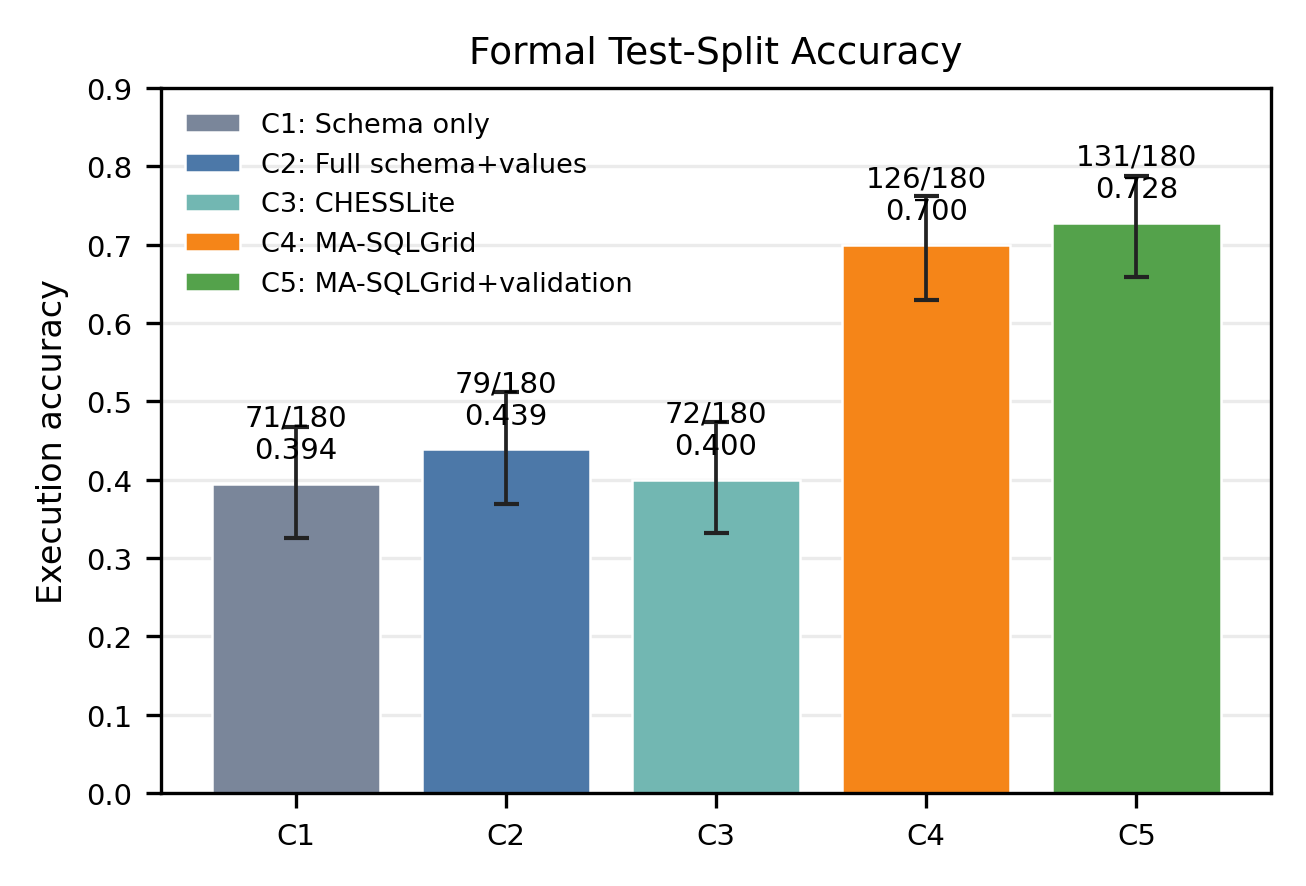
\includegraphics[width=0.95\columnwidth]{charts/fig_main_results.png}
\caption{Formal test-split execution accuracy}
\end{figure}

\begin{figure}
\centering
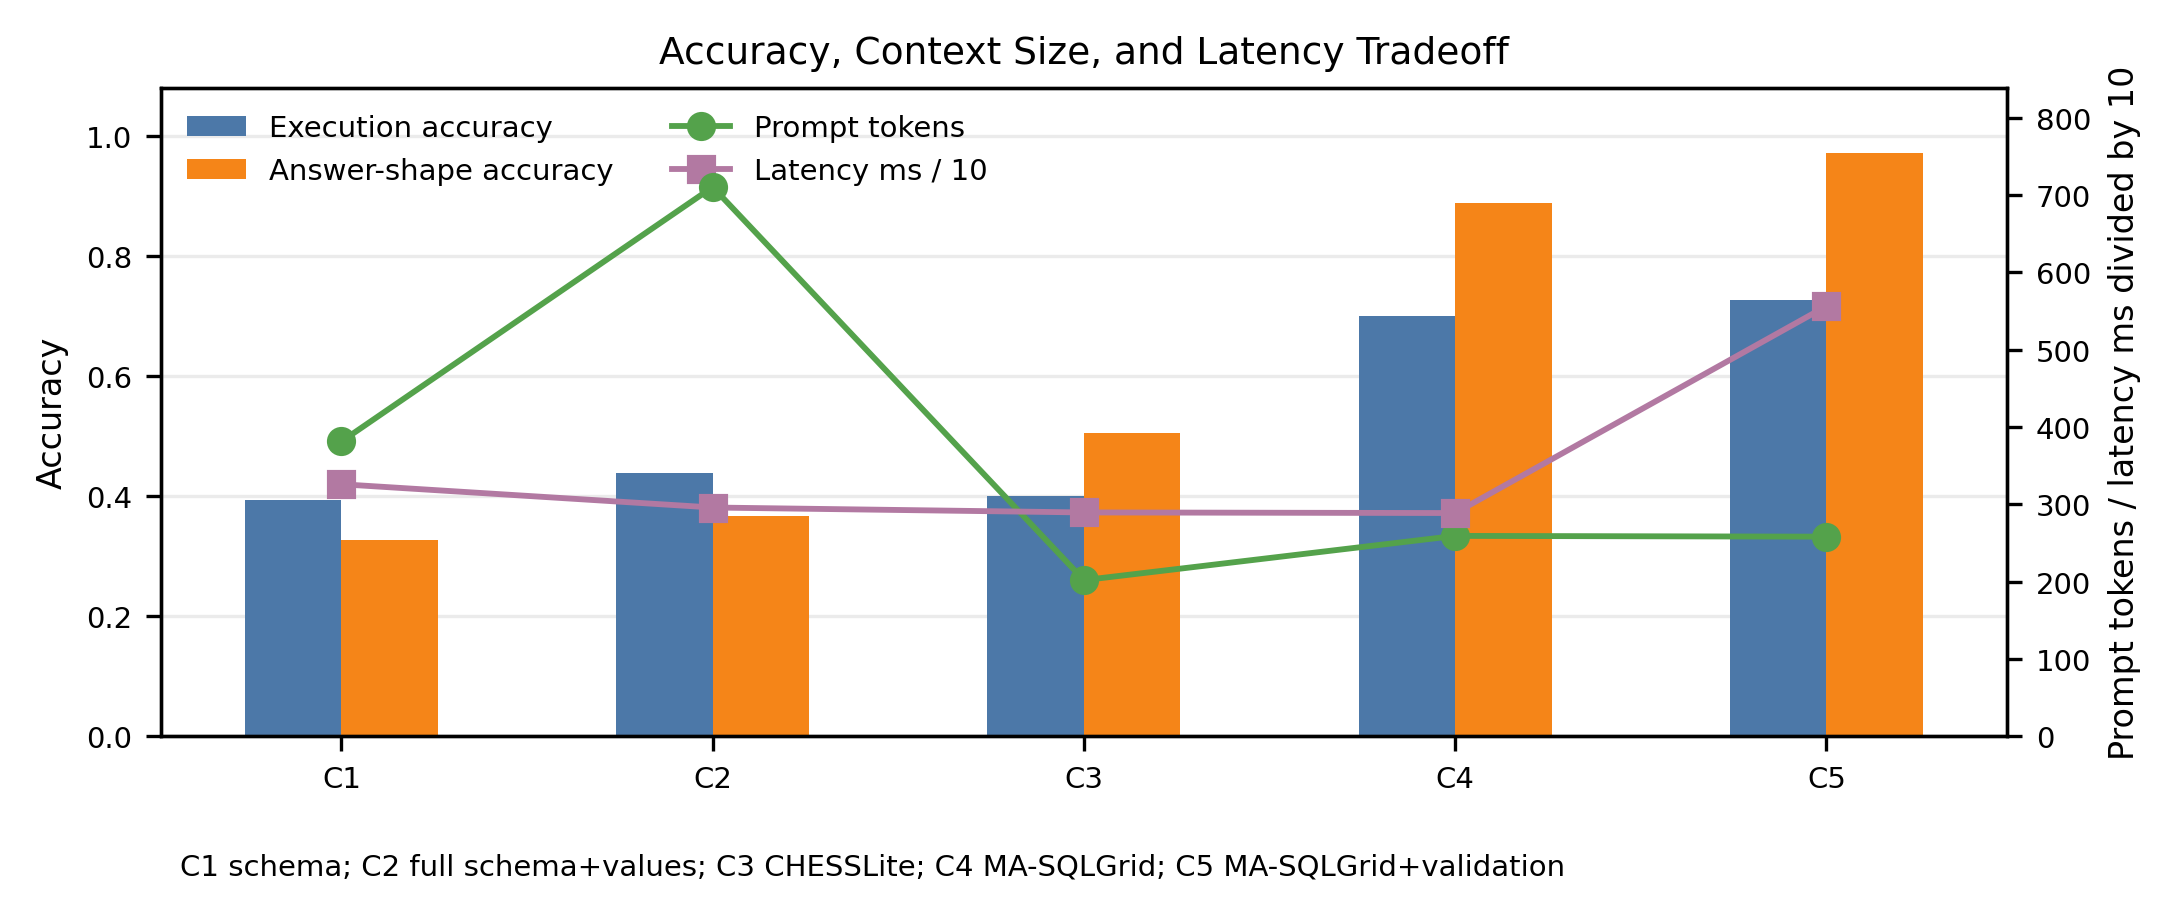
\includegraphics[width=0.95\columnwidth]{charts/fig_multi_metric.png}
\caption{Accuracy, context size, and latency tradeoff}
\end{figure}

The answer-shape metric adds a second layer of interpretation. \texttt{C1} reaches answer-shape accuracy of 0.3278, \texttt{C2} reaches 0.3667, \texttt{C3} reaches 0.5056, \texttt{C4} reaches 0.8889, and \texttt{C5} reaches 0.9722. The shape gain from \texttt{C3} to \texttt{C4} is substantial, which suggests that generic multi-stage prompting is not enough on its own. Shape inference matters most when it is paired with domain normalization. The validated condition then improves shape consistency again, which indicates that validation is not only rejecting invalid SQL but also preferring candidates whose result form matches the question.

Value-hint coverage is treated as an internal trace diagnostic rather than a headline metric. In the runner, a prediction with no inferred value hints receives a vacuous coverage value of 1.0, so this quantity is useful for auditing domain-context traces but not for ranking conditions in the main results table. The stronger evidence for value grounding is instead the paired accuracy gap between \texttt{C4} and \texttt{C2}: the full-schema-values prompt exposes more raw values, but the compact domain context organizes the relevant values around the question, the join path, and the expected answer shape.

The trace-level coverage audit helps interpret this point without changing the main metric. Among the 180 held-out test questions, 170 produced at least one normalized value hint in the domain context. Across those contexts, the runner emitted 330 normalized hint instances and 111 unique rendered hints over 20 matched value columns. These numbers are not used to score predictions, but they show that the normalizer was active on most of the formal split rather than only on a small hand-picked subset.

To separate the two prompt-side components more directly, an addendum run removed one C4 hint channel at a time while preserving the same held-out test split, generator, temperature-zero decoding, and no-gold prediction contract. The addendum does not replace the formal C1--C5 comparison, but it clarifies the mechanism. Removing value hints reduces C4 from 126/180 to 118/180 correct. Removing answer-shape hints reduces it to 77/180 correct and lowers answer-shape accuracy to 0.4389. The result supports a bounded component-level interpretation: value normalization contributes a measurable additional gain, while answer-shape hints are a central part of the compact-context effect on this benchmark.

\begin{table*}[t]
\caption{Bounded in-domain C4 component ablation addendum on the same 180-question test split.}
\centering
\small
\begin{tabular*}{\textwidth}{@{\extracolsep{\fill}}lrrrrr}
\toprule
Condition & Correct & Execution accuracy & Safe SQL & Answer-shape accuracy & Provider failure \\
\midrule
C4 compact domain context & 126/180 & 0.7000 & 1.0000 & 0.8889 & 0.0000 \\
C4 without value hints & 118/180 & 0.6556 & 1.0000 & 0.9167 & 0.0056 \\
C4 without shape hints & 77/180 & 0.4278 & 1.0000 & 0.4389 & 0.0000 \\
\bottomrule
\end{tabular*}
\end{table*}

\subsection{Second-Generator Validation}\label{second-generator-validation}

The second-generator protocol described in Section~5 re-ran C2, C4, and C5 with \texttt{deepseek-chat} on the same 180 held-out test questions using the byte-identical archived prompts and the same packaged evaluator. Table~\ref{tab:second-model} reports the strict and relaxed metrics for both generators side by side; the archived \texttt{gpt-5.4-mini} rows repeat Table~\ref{tab:relaxed-metrics} unchanged.

\begin{table*}[t]
\caption{Cross-model comparison on the 180-question test split under the strict and relaxed metrics. The \texttt{gpt-5.4-mini} rows are the archived formal-run values from Table~\ref{tab:relaxed-metrics}; the \texttt{deepseek-chat} rows come from the second-generator run with byte-identical prompts, temperature 0, and the same evaluator.}
\label{tab:second-model}
\centering
\small
\begin{tabular*}{\textwidth}{@{\extracolsep{\fill}}llrrr}
\toprule
Generator & Condition & Strict (primary) & Order-insensitive & Order-insensitive + projection-tolerant \\
\midrule
\texttt{gpt-5.4-mini} & C2 & 0.4389 (79/180) & 0.4778 & 0.8722 \\
\texttt{gpt-5.4-mini} & C4 & 0.7000 (126/180) & 0.7444 & 0.7444 \\
\texttt{gpt-5.4-mini} & C5 & 0.7278 (131/180) & 0.7722 & 0.8056 \\
\midrule
\texttt{deepseek-chat} & C2 & 0.3389 (61/180) & 0.3667 & 0.8500 \\
\texttt{deepseek-chat} & C4 & 0.7000 (126/180) & 0.7944 & 0.7944 \\
\texttt{deepseek-chat} & C5 & 0.7667 (138/180) & 0.8278 & 0.8278 \\
\bottomrule
\end{tabular*}
\end{table*}

Three findings replicate. First, the compact-context gain replicates and is larger on the second generator: C4 improves over C2 by +36.1 points strict execution accuracy (0.3389 to 0.7000) on \texttt{deepseek-chat}, versus +26.1 points (0.4389 to 0.7000) on \texttt{gpt-5.4-mini}. The C4 strict score is coincidentally identical on both generators (126/180). Second, the validation-layer gain replicates and is also larger: C5 adds +6.7 points over C4 (0.7000 to 0.7667) versus +2.8 points on the original generator. Third, and most importantly for the interpretation in Section~\ref{evaluation-convention-sensitivity}, the projection-tolerant reversal replicates: under the fully projection-tolerant reading, C2 exceeds C4 on both generators (0.8500 versus 0.7944 on \texttt{deepseek-chat}; 0.8722 versus 0.7444 on \texttt{gpt-5.4-mini}), while the compact conditions gain nothing from projection tolerance (C4 and C5 are unchanged on \texttt{deepseek-chat}). The conclusion that the strict gain is dominated by answer-contract conformance rather than row-content retrieval is therefore a cross-model result, not a single-model observation.

\begin{table*}[t]
\caption{Measured resource consumption per question for the \texttt{deepseek-chat} second-generator run (provider-reported usage; direct endpoint with negligible fixed serving overhead). C5 combines candidate generation and, when triggered, one repair call.}
\label{tab:deepseek-tokens}
\centering
\small
\begin{tabular*}{\textwidth}{@{\extracolsep{\fill}}lrrrrr}
\toprule
Condition & Input tokens (mean) & Output tokens (mean) & Latency ms (mean) & Latency ms (median) & First-attempt calls \\
\midrule
C2 & 2011.6 & 49.9 & 1051.9 & 1021.0 & 180/180 \\
C4 & 509.3 & 46.6 & 1054.0 & 1003.5 & 180/180 \\
C5 & 680.5 & 186.2 & 3014.2 & 1965.5 & 178/180 \\
\bottomrule
\end{tabular*}
\end{table*}

Table~\ref{tab:deepseek-tokens} reports the resource profile of the second-generator run. Because the direct endpoint adds almost no fixed per-call overhead, the measured input tokens track the rendered prompts closely: C4 consumes 509.3 input tokens per question against 2011.6 for C2, a 74.7\% measured reduction, consistent in magnitude with the 63.5\% template-level estimate, whereas the original serving stack showed only 23.4\% because of its roughly 4{,}500--4{,}600-token fixed overhead per call (Table~\ref{tab:real-tokens}). The output-side pattern of the original run also replicates: C5 consumes about four times the completion tokens of C4 (186.2 versus 46.6) and roughly triples mean latency (3014.2 versus 1054.0~ms), which is the direct cost of multi-candidate validation. C2 and C4 completed all 360 calls on the first attempt; C5 required a single retry on 2 of 180 questions. The full three-condition run consumed 576.3k input and 50.9k output tokens over 540 calls, with zero provider errors.

The companion consistency check bounds run-to-run variation directly: C4 and C5 were each run three times at temperature 0 (1{,}080 calls total). Per-repeat strict execution accuracy was 0.7056/0.6944/0.7000 for C4 and 0.7667/0.7667/0.7611 for C5, a maximum spread of 1.1 points. Exact SQL string agreement across all three repeats was lower (82.2\% of questions for C4, 77.2\% for C5), confirming that token-level sampling nondeterminism exists on hosted endpoints even at temperature 0; however, all three repeats produced the same correct/incorrect verdict on 98.3\% of questions in both conditions. Combined with the trace-level evidence from the original run (898/900 first-attempt calls at temperature 0), the aggregate metrics and per-question verdicts reported in this paper are highly stable under repetition, even though individual SQL strings are not guaranteed to be byte-identical across runs.

The boundary of this validation should be stated as precisely as the result. The study now covers two generator families, one closed (\texttt{gpt-5.4-mini}) and one open-weight served through its provider endpoint (\texttt{deepseek-chat}); no third family was tested, and the cross-model comparison is at the aggregate level, with no per-question significance test across models. The C5 stage for the second generator is a specification-faithful reimplementation validated at 98.8\% selection agreement against the archive, not the original binary. Within those bounds, every headline effect of the paper replicates with the same sign and larger magnitude.

\subsection{Scale Robustness on the Second Generator}\label{scale-robustness}

The v0.1 database is deliberately small, so a natural objection is that both the accuracy gains and the token economics might be artifacts of a database whose entire value dictionary fits in one prompt. To test this, a deterministic tenfold-scaled variant of the database (\texttt{griddb\_maintenance\_v2\_x10}) was built: every entity table receives ten times the rows (for example, 180 assets instead of 18), and two distractor tables (\texttt{vegetation\_inspections} and \texttt{spare\_parts\_inventory}) are added to the schema. The 180 test questions and their gold SQL are byte-identical to v0.1, and all 200 gold queries were re-validated against the scaled database before any model call (zero gold-validation errors). Because the original \texttt{gpt-5.4-mini} serving stack is no longer available, this experiment is framed as \emph{scale robustness on the second generator}: the C2, C4, and C5 conditions were re-run with \texttt{deepseek-chat} at temperature 0 on the scaled database and compared against the same generator's v0.1 run from Table~\ref{tab:second-model}. The condition contexts were rebuilt with the original context-builder modules received from the experiment machine after the initial release; as a fidelity check, on the v0.1 database those builders reproduce the archived formal-run prompts byte-for-byte (180/180 for both C2 and C4). The run comprised 540 primary calls plus 13 bounded repair calls with zero provider errors and a safe-SQL rate of 1.0 in all conditions.

\begin{table*}[t]
\caption{Scale robustness on \texttt{deepseek-chat}: v0.1 versus the tenfold-scaled (x10) database on the byte-identical 180-question test split, under the strict metric and the order-insensitive projection-tolerant metric of Section~\ref{evaluation-convention-sensitivity}.}
\label{tab:x10-comparison}
\centering
\small
\begin{tabular*}{\textwidth}{@{\extracolsep{\fill}}lrrrr}
\toprule
Condition & Strict v0.1 & Strict x10 & Projection-tolerant v0.1 & Projection-tolerant x10 \\
\midrule
C2 & 0.3389 (61/180) & 0.3333 (60/180) & 0.8500 & 0.8167 \\
C4 & 0.7000 (126/180) & 0.5944 (107/180) & 0.7944 & 0.6944 \\
C5 & 0.7667 (138/180) & 0.6500 (117/180) & 0.8278 & 0.7000 \\
\bottomrule
\end{tabular*}
\end{table*}

\begin{table*}[t]
\caption{Input-token economics at scale (\texttt{deepseek-chat}, provider-reported means per question). The C5 rows include repair calls when triggered.}
\label{tab:x10-tokens}
\centering
\small
\begin{tabular*}{\textwidth}{@{\extracolsep{\fill}}lrrrrr}
\toprule
Condition & Input tokens v0.1 & Input tokens x10 & Growth & Output tokens x10 & Latency ms x10 \\
\midrule
C2 & 2011.6 & 3042.6 & +51\% & 48.6 & 989.7 \\
C4 & 509.3 & 504.0 & $-$1\% (flat) & 47.3 & 1115.9 \\
C5 & 680.5 & 560.5 & $-$18\% & 180.3 & 1834.1 \\
\bottomrule
\end{tabular*}
\end{table*}

Table~\ref{tab:x10-comparison} shows that the two headline effects survive the tenfold scaling. The compact-context advantage persists at +26.1 points strict (C4 0.5944 versus C2 0.3333), attenuated from +36.1 points at v0.1, and the validation layer still adds +5.6 points (C5 0.6500 versus C4 0.5944, versus +6.7 at v0.1). The convention-sensitivity pattern of Section~\ref{evaluation-convention-sensitivity} also persists: C2's failures remain overwhelmingly projection/shape errors (99 of its 120 strict errors are shape mismatches), so under the projection-tolerant reading C2 again overtakes the compact conditions (0.8167 versus 0.6944/0.7000), exactly as at v0.1.

The token-economics contrast in Table~\ref{tab:x10-tokens} is the clearest scale result. The C2 full-schema-values prompt grew by 51\% in measured input tokens (2011.6 to 3042.6 per question) at ten times the rows plus two distractor tables, and it must keep growing with database size because it enumerates the schema DDL and the full value dictionary. The C4 compact context stayed flat (509.3 to 504.0), making compact grounding roughly six times cheaper in input tokens than full-schema prompting at the x10 scale, with the gap widening as the database grows. The builder-side context estimates show the same divergence: the C2 context grows from 631 to 1125 estimated tokens (+78\%) while the C4 context stays at 174 to 176.

The absolute C4/C5 drop from v0.1 requires an honest diagnosis, and the archived traces localize it precisely to a value-inventory truncation artifact rather than a failure of compact grounding. The pilot builder's value inventory enumerates \texttt{SELECT DISTINCT} values per column with an alphabetical \texttt{LIMIT 80} cap. At v0.1 all 18 asset names fit; at x10 there are 180 distinct \texttt{asset\_name} values and the alphabetical top-80 cuts off before the RL-*/SB-*/TX-* names, including the TX-001 to TX-004 literals referenced by test questions, so the affected questions lose their matched-value lines and normalization hints. The decomposition is exact: 149 of the 180 C4 prompts are byte-identical between v0.1 and x10, and on those the x10 run scores 101/149 against 102/149 for the v0.1 predictions re-scored on the x10 database (no scale effect); the entire drop sits in the 31 changed-prompt questions, which fall from 23/31 to 6/31 correct. Two corroborating observations complete the picture. First, C5's repair trigger fires less often at x10 (13 versus 52 repairs) because fewer inferred value hints means fewer missing-value-hint flags, a downstream symptom of the same truncation. Second, re-scoring the v0.1 predictions on the x10 database moves C4 only from 0.7000 to 0.6944 and leaves C5 at 0.7667, so the v0.1 numbers were not inflated by coincidental denotation matches on tiny tables.

Two caveats bound this experiment. First, the two distractor tables stress only C2, whose prompt includes their DDL and values: the C4/C5 builders enumerate a fixed eight-table catalog, so the distractors are excluded from the compact context by construction, not by learned schema selection. Second, part of C4's token boundedness comes from the same \texttt{LIMIT 80} cap that causes the accuracy artifact; the compact context is bounded partly at the cost of value recall. The implication for the method is concrete: the domain-context \emph{idea} survives scale, but the pilot's fixed-cap alphabetical value scan does not, and a deployment-grade version needs a scalable value index (for example CHESS-style keyword or hash-based value retrieval \cite{talaei2024chess}) once a column exceeds roughly 80 distinct values. Section~\ref{limitations} records this as a limitation.

\subsection{Case Analysis}\label{case-analysis}

Three cases drawn verbatim from the archived traces illustrate the mechanism, the value of validation, and its boundary.

\textbf{Case 1 (contract enforcement, Q021).} The question asks: ``Which assets are offline?'' The gold query returns one column, \texttt{asset\_name}, filtered by \texttt{assets.status = 'offline'} and ordered by asset name. The full-schema-values baseline generates \texttt{SELECT asset\_name FROM assets WHERE status = 'offline';}; it uses the right predicate but omits the required deterministic ordering and is scored as a denotation mismatch under the order-sensitive evaluator. The compact domain context records the normalized hint \texttt{assets.status = "offline"} and an inferred shape with one projected column, multi-row output, and required ordering. Under that context, \texttt{C4} generates \texttt{SELECT asset\_name FROM assets WHERE status = 'offline' ORDER BY asset\_name;}, while \texttt{C5} generates the equivalent aliased form. Both match the validated denotation. This is the modal pattern behind the strict-metric gap and is exactly the contract-conformance effect quantified in Section~\ref{evaluation-convention-sensitivity}.

\textbf{Case 2 (execution-guided reranking, Q110).} The question asks: ``List work orders linked to asset REL-002.'' The first C5 candidate, \texttt{SELECT wo.work\_order\_id, wo.status, wo.schedule FROM work\_orders AS wo JOIN assets AS a ON wo.asset\_id = a.asset\_id WHERE a.asset\_name = 'REL-002' ORDER BY wo.work\_order\_id;}, references the nonexistent column \texttt{wo.schedule} and fails execution. The reference-free ranker demotes it and selects the second candidate, a subquery formulation projecting \texttt{work\_order\_id}, \texttt{priority}, and \texttt{status}, which executes and matches the gold denotation. Under C4, which returns only the first formulation, this question is lost. This is the recovery mode that explains most of C5's reduction of execution errors from 20 to 5.

\textbf{Case 3 (repair success and failure on one question family, Q161 versus Q156/Q157/Q158/Q160/Q162).} Six test questions share the template ``Which work orders are assigned to technician \emph{X}?'' The compact context for these questions selects \texttt{work\_orders(work\_order\_id, asset\_id, assigned\_technician\_id, priority, status)} but omits the \texttt{scheduled\_date} column, while the shape hint asks the model to project \texttt{work\_order\_id}, \texttt{status}, and \texttt{scheduled\_date} and the table comment mentions ``schedule.'' Given this inconsistent evidence, the generator hallucinates \texttt{wo.schedule\_date} (or \texttt{wo.schedule}) in every candidate. For Q161 the single bounded repair call, prompted with the execution error, rewrites the column to the correct \texttt{scheduled\_date} and the repaired query matches the gold denotation. For the other five questions the repair reproduces the same nonexistent column and is rejected, leaving the execution error in place; these five are exactly the residual C5 execution errors in the taxonomy table. The family shows both faces of bounded repair: it can fix a locally diagnosable naming error, but it cannot reliably recover information that the compact context itself dropped, since the repair prompt reuses that same context. The root cause is a schema-selection miss, which is why the paper attributes the main effect to context construction and treats validation as a bounded second layer.

\subsection{Tag-Level Diagnostic Breakdown}\label{tag-level-diagnostic-breakdown}

The existing question annotations make it possible to compute a lightweight tag-level diagnostic without rerunning the model. The tag table reports execution accuracy for selected overlapping SQL feature tags. Because questions can have multiple tags, the rows are not disjoint and should not be interpreted as a causal ablation. They nevertheless indicate where compact domain grounding is most useful.

\begin{table*}[t]
\caption{Execution accuracy by question tag using existing formal-run logs. Rows are overlapping diagnostic subsets.}
\centering
\small
\begin{tabular*}{\textwidth}{@{\extracolsep{\fill}}lrrrrr}
\toprule
Tag & Test questions & C2 & C4 & C5 & C4--C2 \\
\midrule
Join & 102 & 0.382 & 0.598 & 0.657 & +0.216 \\
Aggregation & 59 & 0.847 & 0.847 & 0.831 & +0.000 \\
Order-by & 114 & 0.132 & 0.535 & 0.596 & +0.404 \\
Top-k & 18 & 0.000 & 0.889 & 0.833 & +0.889 \\
Time predicate & 30 & 0.000 & 0.533 & 0.567 & +0.533 \\
Group-by & 12 & 0.417 & 0.333 & 0.417 & -0.083 \\
Topology traversal & 11 & 0.091 & 0.818 & 0.909 & +0.727 \\
Self-join & 9 & 0.111 & 0.889 & 1.000 & +0.778 \\
Filter & 170 & 0.441 & 0.718 & 0.753 & +0.276 \\
\bottomrule
\end{tabular*}
\end{table*}

The largest diagnostic gains appear on order-sensitive, top-k, time-predicate, topology, self-join, and filter-tagged questions. Aggregation is not a main source of improvement in this run, and group-by remains mixed. This pattern is consistent with the mechanism: MA-SQLGrid helps most when the question requires the correct literal, projection, ordering, and join path, rather than when a simple aggregate already follows from the prompt.

\subsection{Evaluator-Level Error Analysis}\label{evaluator-level-error-analysis}

The available formal artifacts provide an evaluator-level primary error taxonomy for each condition. This taxonomy is not the same object as the answer-shape accuracy metric reported above. Answer-shape accuracy is a diagnostic rate computed over predictions, while the taxonomy assigns an incorrect prediction to a primary evaluator error category. Likewise, the execution-error column is not a contradiction of the safe-SQL rate: those queries pass the read-only guard but fail when executed against the SQLite schema. The table should therefore be read as a compact view of residual failure labels, not as a complete operator-by-operator causal analysis and not as a replacement for the separate shape metric.

\begin{table*}[t]
\caption{Residual error taxonomy from the archived formal run. Counts are over 180 test questions.}
\centering
\small
\begin{tabular*}{\textwidth}{@{\extracolsep{\fill}}lrrrr}
\toprule
Condition & Correct & Shape mismatch & Wrong denotation & Execution error \\
\midrule
C1 & 71 & 95 & 14 & 0 \\
C2 & 79 & 90 & 11 & 0 \\
C3 & 72 & 67 & 26 & 15 \\
C4 & 126 & 0 & 34 & 20 \\
C5 & 131 & 0 & 44 & 5 \\
\bottomrule
\end{tabular*}
\end{table*}

The first pattern is the reduction of primary shape-mismatch failures after domain-grounded prompting. \texttt{C1} and \texttt{C2} both produce many incorrect queries whose primary failure label is shape mismatch: 95 and 90 cases, respectively. \texttt{C3} reduces that count to 67, which indicates that generic CHESS-style prompting already helps with structural intent. \texttt{C4} and \texttt{C5} have no residual errors whose primary taxonomy label is shape mismatch, while their separate answer-shape diagnostic remains below 1.0000. The combined interpretation is narrower than saying shape problems disappear: the dominant labeled failure mode shifts away from shape mismatch, but some predictions can still have imperfect shape diagnostics or wrong denotations.

The second pattern is the tradeoff between grounding and validation. \texttt{C4} has 34 wrong-denotation errors and 20 execution errors. \texttt{C5} reduces execution errors to 5, which is consistent with reference-free execution validation, but it has 44 wrong-denotation errors. This is plausible for a validator that can reject non-executing candidates and prefer shape-compatible outputs but cannot use gold denotation feedback. It can improve executable consistency and answer shape, yet still choose an executable SQL query that returns the wrong rows. This supports the paper's interpretation of C5 as a modest validation/reranking extension rather than the main mechanism. The main mechanism remains C4's compact domain context, because that is where the large jump over C2 occurs.

The C5 traces make this validation behavior more concrete. Across 180 test questions, C5 selected a non-first candidate in 22 cases. The repair prompt produced a nonempty response in 16 cases, and 15 repaired SQL strings became the final selection. The final selected SQL passed the read-only guard in 180/180 cases, executed in 175/180 cases, matched the inferred answer shape in 175/180 cases, and satisfied the inferred ordering check in 180/180 cases. The remaining five execution failures are not broad safety failures; all are nonexistent-column errors caused by schedule-field naming, with four \texttt{wo.schedule\_date} errors and one \texttt{wo.schedule} error. This explains why validation improves executable consistency but does not eliminate denotation errors.

An offline ranker-weight diagnostic was computed from the archived C5 candidate and validation traces to check whether the conclusion depends on one fragile integer-weight setting. This diagnostic is not a new method selection step and was not used to tune the reported C5 policy. Recomputing the default policy changed 3/180 selected candidates and yielded 132/180 correct, while removing the shape term also yielded 132/180; removing order and empty-result terms yielded 131/180, and execution-only or no-value-term variants yielded 136/180. The range is narrow enough to support the paper's main interpretation: validation is a modest selector over already generated candidates, not the source of the large C4-over-C2 mechanism gain.

The third pattern concerns the role of value information. \texttt{C2} exposes the full value dictionary, but it remains at 0.4389 execution accuracy and still has 90 shape mismatches. This shows that broad value exposure alone does not solve the benchmark. \texttt{C4} uses far fewer prompt tokens and reaches 0.7000, indicating that value evidence must be selected and organized around the question rather than merely listed. The dataset characterization above explains why: most questions combine filters, joins, ordering, and domain literals. A full value dictionary may include the correct literal but still fail to connect it to the correct table, predicate, and answer shape.

The error taxonomy also defines the limits of the current evidence. The dataset annotations show that query families such as joins, aggregations, time predicates, topology traversal, and self-joins exist, but the verified formal artifacts do not provide a per-operator correctness table. The paper therefore does not claim that a specific operator family caused the gain. It claims only what the audited evidence supports: the primary error profile shifts by condition, compact domain grounding produces the main accuracy improvement, and validation reduces some execution and shape-selection failures while leaving denotation errors.

\subsection{Claim-to-Evidence Mapping}\label{claim-to-evidence-mapping}

The main claims are intentionally narrow and map directly to the archived run artifacts released with the paper. The claim-to-evidence table summarizes the mapping so that the reader can distinguish supported results from limitations.

\begin{table*}[t]
\caption{Claim-to-evidence map for the reported MA-SQLGrid results.}
\centering
\footnotesize
\begin{tabularx}{\textwidth}{p{0.24\textwidth}Xp{0.28\textwidth}}
\toprule
Claim & Supporting evidence & Boundary \\
\midrule
Compact domain context is the main mechanism gain under the strict answer-contract metric & C4 reaches 126/180 and 0.7000 accuracy; C4 vs C2 has 49 C4-only correct cases, 2 C2-only cases, and +0.2611 mean difference & Applies to \texttt{GridDB-Maintenance-v2 v0.1} under the fixed generator and the single archived formal pass; the sensitivity analysis in Section~\ref{evaluation-convention-sensitivity} shows the gain is dominated by projection/ordering contract conformance, not row-content retrieval \\
MA-SQLGrid reduces context relative to full-schema-values prompting & C4 uses 259.2 estimated template tokens versus 710.3 for C2 (63.5\% smaller) while improving strict accuracy from 0.4389 to 0.7000; measured API input falls from 6346.7 to 4859.0 tokens per question (23.4\%) & Template tokens are runner estimates; the measured saving is smaller because a fixed serving-side overhead is shared by all conditions (Table~\ref{tab:real-tokens}) \\
Validation improves the final result modestly & C5 reaches 131/180 and 0.7278; C5 vs C4 has 12 C5-only and 7 C4-only correct cases & C5 over C4 is small and not a strong standalone superiority claim; latency increases to 5562.5 ms \\
Answer-shape hints materially affect C4 generation & Removing C4 shape hints lowers execution accuracy from 126/180 to 77/180 and answer-shape accuracy from 0.8889 to 0.4389 & Same fixed GridDB test split and generator; only the shape-hint channel is removed \\
Value hints add a smaller prompt-side gain & Removing C4 value hints lowers execution accuracy from 126/180 to 118/180 & One no-value prediction had a provider/extraction failure and was counted as an error; no cross-domain claim is made \\
The result is evidence-faithful and leakage-controlled & 900 predictions/scores, zero contract errors, zero unsafe SQL, zero provider/extraction errors, and zero leakage-scan problems & Does not imply production readiness or external benchmark transfer \\
The main effects replicate on a second independent generator & \texttt{deepseek-chat} with byte-identical prompts: C4 over C2 +0.3611 strict (0.3389 to 0.7000), C5 over C4 +0.0667 (0.7667); projection-tolerant reversal replicates (C2 0.8500 versus C4 0.7944); direct-endpoint input-token reduction 74.7\% & Two generator families only (one closed, one open-weight); aggregate-level comparison with no per-question cross-model significance test; C5 stage reimplemented from specification (98.8\% selection agreement with the archive) \\
The statistical interpretation is bounded & Paired sign tests compare per-question outcomes on 180 test items; seed 0 is a deterministic pass label; three temperature-0 repeats of C4/C5 on \texttt{deepseek-chat} show a maximum accuracy spread of 1.1 points and 98.3\% per-question verdict agreement & Run-to-run stability is measured only for the second generator; no multi-seed study exists for the original generator \\
The compact-context and validation gains persist at tenfold database scale with bounded input tokens & On the x10 database (10x rows, two distractor tables, byte-identical 180 questions), \texttt{deepseek-chat} gives C4 0.5944 versus C2 0.3333 strict (+26.1 points) and C5 0.6500 (+5.6); C4 input tokens stay flat (509.3 to 504.0 per question) versus +51\% growth for C2; rebuilt contexts verified byte-identical to the archive on v0.1 (180/180) & Second generator only (original serving stack unavailable); the C4/C5 absolute drop from v0.1 is entirely attributable to the \texttt{LIMIT 80} value-inventory truncation (byte-identical prompts 101/149 versus 102/149; changed prompts 6/31 versus 23/31); distractor tables stress only C2 because the C4/C5 builders use a fixed eight-table catalog \\
\bottomrule
\end{tabularx}
\end{table*}

The runtime and executable-SQL numbers are also informative. \texttt{C4} is slightly faster than \texttt{C1} and \texttt{C2}, but it has more execution-error labels than the direct baselines because compact grounding sometimes selects a plausible but invalid local column. \texttt{C5} reduces those execution errors from 20 to 5 by executing and ranking multiple candidates, but it is slower for the same reason. That means the validation layer should be interpreted as a precision-oriented option rather than a default. In a setting where correctness outweighs latency, the extra cost is acceptable. In a time-sensitive interactive setting, \texttt{C4} is the stronger choice because it captures most of the gain at nearly the same runtime as the simpler prompts.

Overall, the results support a concise claim. Compact domain grounding is the main driver of improvement, and reference-free validation adds a smaller but measurable second gain. The benchmark is deterministic, the evaluation contract is fixed, and the metric is execution accuracy, so this is the correct level of evidence to report. The paper does not need broader claims to make the result meaningful.

\section{Discussion}\label{discussion}

The main result is that compact, domain-normalized context is more effective than exhaustive schema exposure for this database. That pattern is consistent with prior schema-linking and grounded prompting work, but the present benchmark makes the mechanism unusually clear \cite{lei2020reexamining}, \cite{liu2022semantic}, \cite{quamar2022natural}, \cite{xie2022unifiedskg}. When the schema is frozen, the key question is not how much evidence to include. It is which evidence actually constrains the join path, predicate value, and answer shape. MA-SQLGrid answers that question by selecting a smaller but better aligned prompt, and the execution gain indicates that the generator benefited from that reduction.

A second finding is that answer-shape control matters more when it is coupled to value normalization. The generic CHESS-style baseline improves shape accuracy relative to schema-only prompting, but it does not reach the same execution level as MA-SQLGrid because it lacks the domain-specific canonicalization step \cite{talaei2024chess}, \cite{wang2023macsql}, \cite{pourreza2023dinsql}. The new addendum makes the same point from the opposite direction: removing shape hints causes a large accuracy drop, while removing value hints causes a smaller but still measurable drop. A query can have the right structure and still return the wrong rows if the status or category literal is off by one canonical form; conversely, literal hints are much less useful when the generated SQL has the wrong projection or ordering form.

The validation layer deserves a separate interpretation. Its gain over compact grounding is smaller than the gain from compact grounding over full-schema prompting, which is exactly the pattern a reference-free selector should produce \cite{wang2021executions}, \cite{li2024select}, \cite{huang2024survey}. Validation can clean up remaining shape and value inconsistencies, but it cannot replace good context construction. That is why the validated variant improves answer-shape accuracy most visibly and execution accuracy more modestly. The method therefore behaves as a two-stage system: grounding does the heavy lifting, and validation corrects a subset of residual errors.

The runtime tradeoff is also meaningful. The compact-domain condition is not slower than the full-schema baseline, so the improvement is not bought with a wider prompt. The validated condition is slower because it evaluates multiple candidates, but the latency remains a consequence of the selection policy rather than of the grounding step itself. That distinction matters for deployment. If the task is interactive and latency-sensitive, compact grounding alone is the better choice. If correctness is more important than speed, validation is justified. Prior agentic and execution-guided systems have often emphasized broader search or heavier refinement loops \cite{wang2023macsql}, \cite{pourreza2024chasesql}, but this benchmark suggests that a smaller control loop can be enough when the schema is fixed and the domain vocabulary is narrow.

The broader implication is modest but useful. In tightly scoped operational databases, a compact prompting strategy can outperform a fuller prompt that looks more complete on paper. That is especially relevant for power-grid maintenance tasks, where the schema and value space are regular enough to support selective grounding, but the questions still require careful literal matching and shape control. The results do not justify general claims about all Text-to-SQL settings. They do show that in this setting, compact-domain prompting plus validation is the right design point.

This finding also clarifies how the method should be used. If the user needs a low-latency path, C4 is the preferred condition because it captures the main gain without the validation overhead. If the user can tolerate additional latency for improved answer-shape consistency and a small accuracy gain, C5 is the stronger choice. The paper therefore does not present validation as universally superior. It presents validation as a bounded extension whose value depends on whether the deployment scenario prioritizes execution accuracy or response time. That distinction follows directly from the reported results: C5 is best overall, but the most important scientific result is the C4 jump over the non-MA-SQLGrid baselines.

Finally, the study suggests a practical design rule for similar fixed-schema databases. The first priority should be to identify the domain vocabulary and answer forms that repeatedly appear in user questions. Only after that context is reliable should validation be added. A validator over poorly grounded candidates may reduce syntax and shape failures, but it cannot reliably recover missing domain evidence. In contrast, a compact context that already captures the relevant value and shape information gives the validator candidates worth selecting. This staged interpretation is what makes MA-SQLGrid more than a prompt-length comparison: it ties the improvement to a sequence of schema selection, value normalization, shape control, generation, and reference-free selection.

\section{Limitations}\label{limitations}

This study is tied to a single synthetic and deterministic maintenance database, so the results should be read as evidence about this benchmark rather than a general statement about all enterprise schemas. The split is fixed, the value space is frozen, and the query family is controlled, which makes the dataset well suited to testing grounding and validation but narrow in scope \cite{zhong2020semantic}, \cite{lei2024spider}. The original formal run uses one deterministic pass; run-to-run variation is bounded empirically only for the second generator, through the three-repeat consistency check in Section~\ref{second-generator-validation}, and no multi-seed study exists for the original generator.

The generators are hosted models: one closed non-frontier model (\texttt{gpt-5.4-mini}) and one open-weight model family served through its provider endpoint (\texttt{deepseek-chat}). Although both runs archive prompts, hashes, selected outputs, raw responses, traces, and serving metadata, exact reproduction may be affected if a hosted implementation changes after the experiment. The claims are therefore tied to the archived run packages and model identifiers, not to an assumption that a future endpoint invocation will be byte-identical. The second-generator validation also has its own limits: it covers only one additional model family, the cross-model comparison is aggregate-level with no per-question significance test across models, and the C5 stage for the second generator is a specification-faithful reimplementation (validated at 98.8\% selection agreement with the archive) rather than the original binary.

The validated condition adds a real latency cost because it executes and scores multiple candidates before choosing one. That overhead is visible in the reported runtime and is the main practical tradeoff of the method. The paper reports tag-level diagnostics and bounded value/shape ablations, but it does not include a full causal operator-by-operator ablation or a schema-drift stress test. Those analyses would require additional experiments that were not conducted on the verified benchmark.

The scale-robustness experiment of Section~\ref{scale-robustness} has its own boundaries. It was run only on the second generator, because the original \texttt{gpt-5.4-mini} serving stack is no longer available, so it bounds scale behavior for the \texttt{deepseek-chat} replication rather than for the archived original run. Its diagnosis also exposes a genuine implementation limitation: the compact context's value inventory enumerates at most 80 distinct values per column in alphabetical order, which silently drops question-relevant literals once a column exceeds that cap, and the entire C4/C5 accuracy drop at tenfold scale is attributable to this truncation. The compact context is therefore bounded partly at the cost of value recall, and a deployment-grade version should replace the fixed-cap scan with a scalable value index, for example CHESS-style keyword or hash-based value retrieval \cite{talaei2024chess}. Finally, the two distractor tables stress only the full-schema condition, because the C4/C5 builders enumerate a fixed eight-table catalog; the experiment therefore does not measure learned schema selection under schema growth.

Another limitation is that the implementation is evaluated as a complete pipeline rather than as a fully randomized component study. The C1-C5 conditions and addendum ablations isolate major design choices, but they do not independently randomize every rule used in schema selection, value normalization, answer-shape inference, and validation. The evidence is therefore strongest for the system-level comparison and for the two removed hint channels, and weaker for fine-grained causal claims about each internal rule. This is why the paper frames C4 as the main mechanism evidence and treats the internal diagnostics as explanations of the observed behavior, not as separate proofs of every component.

\section{Conclusion}\label{conclusion}

MA-SQLGrid shows that a lightweight multi-stage Text-to-SQL pipeline can improve domain grounding on a fixed power-grid maintenance database. Compact schema/value context, value normalization, and answer-shape inference outperform broader baseline prompting, and reference-free validation adds a smaller final gain. Both effects, and the convention-sensitivity caveat that bounds their interpretation, replicate on a second independent generator with larger margins. A tenfold database-scale stress test on the second generator shows that both gains persist at scale with flat compact-context input tokens, while exposing a fixed-cap value-inventory limitation that future versions should replace with a scalable value index.

The practical takeaway is simple: in a narrow operational database, better context matters more than more context, and most of the measurable benefit comes from making the expected answer contract explicit before generation. Future work should test the same design under schema drift and with generator families beyond the two evaluated here, replace the fixed-cap value inventory with a scalable value index and re-test at larger scales, repeat the evaluation on public benchmarks, expand the error analysis by query type, and evaluate whether compact grounding transfers to other infrastructure databases with similarly structured vocabularies.


\section*{Data Availability}

The artifact package accompanying this paper contains the frozen dataset (\texttt{schema.sql}, \texttt{database.sqlite}, \texttt{questions.jsonl}, \texttt{splits.json}, annotation protocol), the semantic evaluator with unit tests, the per-condition prompts and context hashes, all 900 prediction/score records and raw API traces of the original run, the second-generator (\texttt{deepseek-chat}) prediction/score records and the three-repeat consistency outputs, the tenfold-scaled database with its scale-robustness run outputs and full traces, the original context-builder modules (verified to reproduce the archived formal-run prompts byte-for-byte), the component-ablation and diagnostic outputs, and the analysis scripts that recompute every number reported in this paper from those artifacts. It is publicly available at \url{https://github.com/gaoxingkele/ma-sqlgrid} (release v0.2.0).

\section*{AI Use Disclosure}

Hosted large language models (\texttt{gpt-5.4-mini} and \texttt{deepseek-chat}) are the experimental subjects of this study: they served as the fixed SQL generators whose behavior under different context-construction conditions is measured, and all of their outputs are archived in the released traces. In addition, AI-based writing and coding assistants were used to help draft and edit the manuscript text and analysis code. All experimental numbers were computed from the archived run artifacts, all content was reviewed and verified by the authors, and the authors take full responsibility for the manuscript.

\section*{Funding}

This work was supported by the Science and Technology Project of NARI Group Corporation (State Grid Electric Power Research Institute) (Grant No. [TODO: grant number]).

\section*{Conflicts of Interest}

The authors declare no conflict of interest.

\appendices

\section{Prompt Templates for the Five Conditions}\label{appendix-prompts}

All five conditions share fixed prompt templates; only the context block differs. The templates below are reproduced verbatim from the archived experiment runner, and every rendered prompt (with its hash) is included in the released traces. Placeholders in angle brackets are filled per question.

\subsection{Direct-generation template (C1--C4)}

\begin{small}
\begin{verbatim}
You are a Text-to-SQL system for a synthetic
SQLite power-grid maintenance database.

Return exactly one read-only SQLite SELECT
query. Do not include markdown or explanation.
Do not use INSERT, UPDATE, DELETE, DROP,
PRAGMA, or multiple statements.
Use only the provided database context. When
normalization hints or answer-shape hints are
present, treat them as question-derived
constraints. Match the requested projection
count and include relevant literal predicates.

Condition: <condition name>

<context block>

Question ID: <question id>
Question: <question text>
\end{verbatim}
\end{small}

The context block is the only element that varies across conditions: C1 inserts the full raw \texttt{schema.sql}; C2 inserts a rendered dump of the full schema plus the enumerated distinct values of all non-ID columns; C3 inserts the generically selected schema subset produced by lexical matching without domain rules, value normalization, or shape hints; C4 inserts the compact domain context shown below.

\subsection{Rendered compact domain context (C4/C5), example for Q021}

\begin{small}
\begin{verbatim}
SQLite selected context:
Tables and selected columns:
- asset_types(asset_type_id) -- equipment type
  catalog such as Transformer, Breaker, Line,
  Relay, Substation, Capacitor
- assets(asset_id, asset_name, asset_type_id,
  location_id, status) -- individual grid
  assets with names, type, location, install
  date, status, and MW capacity
- grid_topology(edge_id, upstream_asset_id,
  downstream_asset_id) -- directed
  upstream/downstream asset connections and
  switch status
- locations(location_id) -- grid yards,
  substations, regions, coordinates, and
  location criticality
- sensor_readings(reading_id, asset_id) --
  time-series sensor readings for assets with
  sensor type, value, unit, and alarm flag
- work_orders(work_order_id, asset_id,
  assigned_technician_id) -- maintenance work
  orders with priority, status, schedule,
  completion date, and fault code
Join paths:
- assets.asset_type_id =
  asset_types.asset_type_id
- assets.location_id = locations.location_id
- work_orders.asset_id = assets.asset_id
- sensor_readings.asset_id = assets.asset_id
- grid_topology.upstream_asset_id =
  assets.asset_id
- grid_topology.downstream_asset_id =
  assets.asset_id
Exact database values matched from the
question:
- assets.status: offline
Power-grid domain normalization hints inferred
from the question:
- assets.status = "offline"
Answer-shape hints inferred from the question
text:
- expected column count: 1
- row granularity: multi-row
- deterministic ordering needed: True
- Project asset_name for asset listing
  questions.
\end{verbatim}
\end{small}

\subsection{Candidate-generation template (C5)}

\begin{small}
\begin{verbatim}
You are generating candidate SQLite SQL for
CHESS-style MA-SQLGrid.

Return 3 distinct read-only SQLite SELECT
queries as a numbered list. Do not include
explanation.
Do not use INSERT, UPDATE, DELETE, DROP,
PRAGMA, or multiple statements.
Use only the selected context, normalization
hints, and inferred output-form hints below.
Candidate queries should differ in plausible
joins/projections while respecting the
inferred projection count and relevant literal
predicates.

Condition: <condition name>

<compact domain context block, as in C4>

Question ID: <question id>
Question: <question text>
\end{verbatim}
\end{small}

\subsection{Bounded repair template (C5, at most one call)}

\begin{small}
\begin{verbatim}
Repair this SQLite SELECT query using only
selected context and inferred hints.

Return exactly one read-only SQLite SELECT
query. Do not include markdown or explanation.

<compact domain context block, as in C4>

Question ID: <question id>
Question: <question text>
Previous SQL: <selected candidate SQL>
Reference-free validation result:
<JSON validation record: exec_ok, shape_ok,
order_ok, empty result, matched and missing
value hints>
\end{verbatim}
\end{small}

The repair prompt receives only the reference-free validation signal; it never receives gold SQL, gold rows, evaluator verdicts, or dataset metadata.

\bibliographystyle{IEEEtran}
\bibliography{references_verified}
\EOD
\end{document}
